\documentclass[11pt]{report}

\usepackage{physics}
\usepackage{amsmath,amsfonts,amssymb,amsthm}
\usepackage{braket}
\usepackage{bbold}
\usepackage{hyperref}
\usepackage{enumerate}
\usepackage{gensymb}
\usepackage{siunitx}


\usepackage{fancyhdr}
\usepackage{graphicx}
\usepackage{titlesec}
\usepackage{tabularx}
\usepackage{subcaption}
\titleformat{\chapter}[display]
  {\normalfont\bfseries}{}{0pt}{\huge}
\graphicspath{ {./images/} }
\newcommand{\namespacing}{0.2in}
\newcommand{\mychapter}[2]{
	\setcounter{chapter}{#1}
	\setcounter{section}{0}
	\chapter*{#2}
	\addcontentsline{toc}{chapter}{#2}
}

\begin{document}

	\pagestyle{fancy}
	\fancyhf{}
	\rhead{\dots}
	\lhead{PHAS0052: Physics Group Project}
	
	\begin{center}
	\thispagestyle{empty}
	\vspace*{-2in}
 	\makebox[\textwidth]{
\includegraphics[width=1.1\paperwidth]{banner}} \\[2in]
  	\Huge{Physics and COVID-19} \\[0.5in]
  	\large{Authors} \\[\namespacing]
  	\normalsize{Gustavs Zilgalvis, Alexander Sells, Zaki Salma, Joel Pendleton, Xudong Ke Lin, Indra Gankhuyag, Vincent Denuit} \\[0.2in]
  	\large{Board Member} \\[\namespacing]
   	\normalsize{Stan Zochowski} \\[0.2in]
   	\large{\today}
	\end{center}
	\pagebreak

	\tableofcontents{}
	\mychapter{0}{Executive Summary}
	
	Notes on who has added to each sections so far:
\begin{itemize}
\item{Identification} 
\item{Detection} - Zaki
\item{Testing} -  Sells
\item{Infrared Thermometers} - Sells
\item{Symptoms} - Sells
\item{Characterisation}  - Zaki
\item{Imaging} - Zaki,
\item{Spread}
\item{Containment}
\item{Inactivation} - Vincent,
\item{Masks}
\item{Social Distancing} Vincent
\item{Filtration} - Sells
\item{Eradication}
\item{Vaccines} - Vincent
\item{Treatment} - Gustavs
\item{Ventilators} - Sells
\item{Inactivation II}
\item{Simulations} - Joel, Indra, Xudong
\item{Statistical Analysis}
\end{itemize} 

	\chapter{Preface}
	\chapter{Identification}

Since the Covid-19 pandemic had first surfaced in late 2019, the identification of the virus has proved to be a crucial factor in its containment and an area of great interest within the scientific community as a result of the inherent difficulty in detecting the pathogen (long incubation time, high case to case variation in patient symptoms), as well as its life-saving practical applications.

This section serves to catalogue the various techniques in physics that have played an important role in the identification and characterisation of the virus.

		\section{Detection}	


\subsection{Testing}
Most strategies for reducing the transmission of COVID rely on the mass testing of people for the virus, and any transition to a post-pandemic society is likely to demand a large number of fast and accurate screenings. The majority of COVID tests in the UK are polymerase chain reaction (PCR) tests \cite{testing1}, considered a ‘gold standard’ detection method, and which was already used to detect a wide range of pathogens including HIV \cite{testing2}. However, the process requires swabs to be put through a reverse transcription (RT)-PCR machine, normally located at a lab, and so there is a significant time delay between swab being taken and results being received, particularly when testing is being performed on a large scale.

The introduction of the lateral flow test device (LFD), which is self contained and does not require a laboratory to perform, partly solved this issue. However, tests performed by the UK COVID-19 Lateral Flow Oversight Team on the first antigen LFD to be approved in the UK (Innova) suggested a sensitivity (correctly identified positives) of 78\% when performed by laboratory scientists \cite{testing3}, which was skewed towards the higher viral loads. 

There is therefore demand for a COVID detection method that combines the confidence of the PCR method with the rapidity of the lateral flow device, and a research team from the department of Physics at Oxford University \cite{testing4} is investigating whether labelling virus particles with fluorescent molecules can fulfil these requirements by adding florescent molecules to virus particles.

The method is based on the first study of the phenomenon by Robb et al. (2019) \cite{testing5} and uses a mixture of calcium chloride and a fluorescent (re-emits light upon excitation) DNA molecule, with the calcium ion thought to bind a negatively charged phosphate ion in the DNA strand to the negatively charged surface of a viral capsule, which in the 2019 experiment belonged to an Influenza virus. The DNA was made fluorescent by attaching a widely used labelling molecule known as ATTo 647N, which absorbs light of wavelength 646 nm and emits light of 664 nm (both averages) \cite{testing6}. When many of these fluorescent DNA strands become attached to an individual virus, it becomes bright enough against the free-fluorescent-molecule background to be tracked by a computer as 646 nm light is shone at a sample. By comparing the intensities of light emitted by treated virus particles to the intensity of single fluorescent DNA strands, it was estimated that there were on average 33 DNA strands bound to each influenza virus.

When performing experimental runs in which either the virus, the calcium chloride or the fluorescent DNA was substituted for water, no florescent spots were observed in the images taken of the samples, providing strong evidence that it was indeed the influenza viruses being marked. The researchers devised a further method for verifying that the bright spots in their images were the target virus by using the Stokes-Einstein equation, which can relate the mean diffusion coefficient of a particle to its diameter. The full relation is:

\begin{equation}
    d_{st}=\frac{k_{B}T}{3\pi{}D_{m}\eta}
\end{equation}

Where $d_{st}$ is the Stoke’s diameter, $D_{m}$ is the mean diffusion coefficient, $\eta$ is the viscosity of the liquid and all other factors are conventionally labelled. In order to determine the mean diffusion coefficient, 1000 images of a sample were taken at a rate of 33 Hz, and the paths of each bright spot tracked. Once the average displacement of a particle is determined from each frame, the diffusion coefficient is:

\begin{equation}
    D=\frac{\sqrt{<(\Delta{}x)^{2}>}}{6\Delta{}t\epsilon}
\end{equation}

where $\Delta{}x$ is the displacement, $\Delta{}t$ is the time period and $\epsilon$ is a correction factor recommended for camera based tracking \cite{testing7}. The results showed an average diameter of 134 nm, which was in accordance with measurement using electron microscopy of the influenza which placed most viruses at 120-140 nm in diameter.

Key to this technique’s potential as a COVID diagnostic is its ability to detect the virus at low concentrations. The Oxford study, which used machine learning to detect fluorescently labelled COVID viruses, estimated a limit of detection of $6\times{}10^{4}$ plaque forming units per millilitre (pfu/ml). This is in stark contrast to a recent government trial of the Innova LFD estimating its limit of detection to be 100 pfu/ml \cite{testing8}. However, this should not be immediately used to dismiss florescent DNA marking as a mass testing alternative, as lateral flow tests have been in use for at least 60 years \cite{testing9}, meaning that the technology has had more time to be finely calibrated.

More promising is the sensitivity data, which the same Oxford fluorescent DNA group reported at around 70\% from one test involving clinical COVID-19, whereas the Innova LFD group showed a sensitivity of 78.8\% while detecting COVID-19 infections in a similar laboratory environment. Although the two results can’t be directly compared due to substantial differences in method, they do show that florescent DNA marking has potential to be a successful LFD competitor if this comparable sensitivity can be maintained as a commercial device is manufactured.

Qualitative comparisons can also be made between LFDs and the florescent marking method to predict its suitability as a mass testing device. Like the LFDs, no stages of the florescent marking method required a deviation from room temperature, a key advantage over PCR which requires large oscillations in temperature in order to trigger repeat chemical reactions. In addition the Innova LFD claims to deliver a result in under 30 minutes whilst the recent Oxford florescent marking study reported the ability of its machine learning program to detect a non-specific virus in under 5 minutes. Finally, compared to PCR, the florescent marking technique uses many fewer chemicals since it does not require the processing of samples to extract RNA, suggesting that an eventual florescent marking based test would be much cheaper and therefore more suitable for mass testing than PCR.

The main disadvantage of florescent marking compared to LFDs at this stage is the requirement for a source of laser light to induce the florescence and the computer-based analysis of the light. This suggests a need for at least some ‘infrastructure’ where the test is taken, at the very least a source of electrical power and a capable computer, whereas once an LFD is created the test can arguably be taken anywhere in the world since the device is completely self-contained.

In summary, results at a very early stage in the florescent marking test’s development show that it is an effective way of identifying viruses from clinical samples, and so should be pursued as a testing alternative, particularly when concerns are being raised over the performance of LFDs following their public distribution \cite{testing10}. In addition, having proved to be a fast and inexpensive technique, florescent marking could be a very useful tool at the tail end of the COVID 19 pandemic with the need for sustained mass testing as social restrictions are lifted.  However, due to the current requirement for machinery for the analysis of the tests, any potential roll-out is likely to fill a ‘middle ground’ between PCR and LFDs, being a fast, accurate, inexpensive, non-lab-based test but requiring ‘analysis stations’ with limited mobility. These could be positioned at places where testing is routine such as care homes or hospitals.


 
 
 



			
			\subsection{Symptoms}		

\subsubsection{Infrared Thermometers}
			
The COVID-19 pandemic has seen the widespread deployment of non-contact infrared thermometers (NCITs) in public places to control the spread of the virus. The technology is well established, and has mainly been used to measure temperature in very young children and new-borns where more invasive methods such as taking a reading from inside the mouth can cause discomfort \cite{ir1}. NCITs have also been deployed at airports during previous pandemics such as the Ebola outbreak (2013-16) \cite{ir2} due to the reusability of the devices over many scans and the low risk of transmitting an infection via a device. However, one study of the temperature screening at Freetown international airport in Sierra Leone \cite{ir3} showed that 0.006\% of screened passengers were identified as having a fever by NCITs and none of those were diagnosed with Ebola. At least two passengers screened by NCITs went on to be diagnosed with Ebola in their destination countries. This raises the questions over whether NCITs are effective at identifying infected people when used en masse.

Most NCITs work by measuring the radiance of an object \cite{ir4}. This can be related to temperature through the Stefan-Boltzmann equation:

\begin{equation}
    P_{rad} = \epsilon{}\sigma{}T^{4}
\end{equation}

where P is the power radiated per unit area, $\sigma{}$ is the Stefan-Boltzmann constant, T is the temperature of the object being measured and $\epsilon$ is the emissivity of an object, which for a perfect black body is 1 but for the human body is about 0.98 \cite{ir5}. At normal temperatures most of the black body radiation emitted by the human body is infrared with wavelengths of around 10 $\mu{}m$.

If a device is fitted with a substance that is effective at absorbing such wavelengths, the emitted power can be used to heat a component called a thermocouple. This consists of two wires connected together in a closed circuit, each made of a different metal. Due to different electronic properties of the metals, if one of the connections between them is hotter than the other connection, a potential difference will be generated. NCITs utilise this by having the infrared-absorbent material at one end of the thermocouple and a known ambient temperature at the other. The total power absorbed from the object is then:

\begin{equation}
    P_{rad}=\epsilon{}\sigma{}(T^{4}_{obj}-T^{4}_{amb})
\end{equation}

where ‘obj’ refers to the object being measured and ‘amb’ refers to the known ambient temperature in the device. The voltage induced in the thermocouple is proportional to the power and so this can be measured to calculate the object’s temperature.

Although this design provides numerous strengths, such as being able to measure temperature with some degree of accuracy without having to make contact with a potentially infectious subject, there are some aspects which call into question its reliability on a large scale.

Firstly it should be acknowledged that not all COVID infections present as a fever. For those who show symptoms, a WHO report from China in early 2020 \cite{ir6} reported that 87.9\% of 55924 confirmed cases developed a fever, and in a study in the UK, the number of confirmed positive cases with a fever was as low as 34\% \cite{ir7}, however this study is slightly less reliable as the symptoms were self-reported by patients. Furthermore, the variability in the progression of the disease in different people means that over the roughly two weeks that the disease lasts, a fever may only be present for a certain fraction of the time, meaning symptoms conducive to transmission such as a cough could be present without a detectable rise in body temperature.

In addition, it has been estimated that around 20\% of all infections are completely asymptomatic \cite{ir8}, and that the relative risk of transmission was only about 40\% lower for asymptomatic people, although this figure is still relatively uncertain. Other studies have placed the rate of asymptomatic cases to be about 40\% \cite{ir9}. A large analysis of contact tracing data in Hunan province in China also estimated that 60\% of transmission occurred when infected individuals were pre-symptomatic \cite{ir10}. In all of these cases an NCIT would have a very low chance of detecting an infected individual.

These data immediately suggest that on its own, measuring temperature is not a robust way of identifying COVID cases, especially when compared with mass testing devices such as the lateral flow test, which tests specifically for the virus and therefore theoretically has a chance of identifying every positive case rather than NCITs which test for a symptom which may not be present.

It must also be assumed that infrared thermometers have an automatic temperature adjustment or very clear instructions on what constitutes a fever since normal forehead temperature is different from normal ‘core temperature’, and while the former lies between 31.0 and 35.6 degrees Celsius \cite{ir11}, most medical advice generalises a fever as a temperature above about 38 degrees Celsius such as the NHS website \cite{ir12}, which is far beyond the fever temperature of a forehead at 35.6 degrees Celsius.

The next factor to consider is the accuracy of the devices when used on infected people who do have a fever. One study in 2015 found that one NCIT had only a 29.4\% sensitivity rate \cite{ir13}, but it should be noted that this study was conducted in Singapore and the paper only discouraged its use in tropical climates. The higher ambient temperature may raise the ambient temperature of the thermocouple to a point where it becomes less accurate.

A further variable is the effect of different skin surfaces. A study comparing different temperature measurements in individuals who were exercising found that at the onset of sweating, infrared thermometry readings started decreasing whilst rectal and oesophageal temperature was increasing \cite{ir14}. This was attributed to the layer of sweat cooling down the skin relative to the core body temperature and also affecting the emissivity of the skin.

A study in South Korea by Zheng et al. (2020) \cite{ir15} investigated the effects of ten different cosmetics on the reliability of NCITs. Most of the products decreased the temperature measurement, with the largest decrease of 2 degrees Celsius being observed in the first fifteen minutes after application of a ‘tone up brightening cream’. After 40 minutes the skin was washed and measured again which showed that the temperature was still depressed by 0.8 degrees Celsius. The study suggested three main mechanisms that caused the temperature reading to drop after application of the products which were: evaporative cooling of the skin from volatile liquids, substances on the outside of the skin acting as a barrier to the skin’s radiation, and solids in the products that reduce the skin’s emissivity. The authors concluded that common cosmetics could easily reduce an IR temperature reading by up to 2 degrees Celsius.

On top of cosmetics there are numerous variables that could have a further effect such as the presence of wind, the level of cleanliness of the skin and level of mental stress. Finally, many infrared thermometers have a specific distance that they must be measured at, for example the manual for the PC868 NCIT states that measurement should be taken from a distance of 3-5 cm from the forehead \cite{ir16}. However a combination of scans being performed by non-medically trained individuals and government advice to keep a 2 m distance from other people could lead to temperatures being taken from further away, resulting in an underestimate of forehead temperature due to less radiation reaching the device.

To summarise, it is overwhelmingly evident that NCITs are not an effective way of stopping the spread of COVID-19, based on the limited probability than an infection risk is displaying fever symptoms at the time of measurement, and the number of variables that could affect the accuracy of the reading. This conclusion is backed up by official government advice against using them to detect COVID \cite{ir17}. Despite this, provided that all participants are aware of the high chance of a false negative result, there are few health risks associated with using an infrared thermometer. Therefore it is not unreasonable to use NCITs as a supplement to more reliable screens such as lateral flow antigen tests for travellers since they are cheap and reusable. However, using only NCITs as a way of testing people for COVID before they enter a social venue such as a pub would not be effective at stopping the spread. The role of NCITs at the tail end of the pandemic is therefore small, and due to their widespread availability and use it is important to provide information about their potentially misleading results when used to test for COVID.

\medskip





		\section{Characterisation}




			\subsection{Imaging}
			
			Virus imaging techniques aid researchers in better understanding the structure and features of the SARS-CoV-2 virus which causes Covid-19 disease.			


\subsubsection{Producing X-rays}

X-rays are used in a multitude of viral detection techniques, this section will outline the different methods in their production and the advantages of these approaches.

\subsubsection{The X-ray tube}

The X-ray tube is a device which is composed of a cathode and an anode in a vacuum tight glass envelope  (See Figure 2). An electric current is passed through the cathode, typically a tungsten filament, causing it to emit electrons which travel towards the anode.

\begin{figure}[h!]
\centering
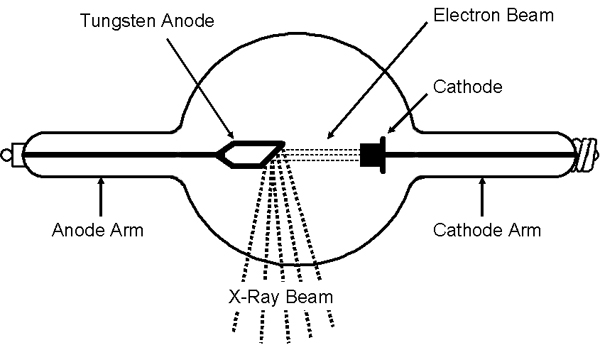
\includegraphics[scale=0.4]{X-ray Tube image.jpg}
\caption{Schematic of the inside of a X-ray tube \cite{xraytubediag}[7].}
\label{2}
\end{figure}

As these high speed electrons approach the anode, they decelerate due to a repulsion force from the electrons in the material of the anode. The deceleration of a moving charge results in Bremsstrahlung or breaking radiation giving rise to a continuous X-ray spectrum closely described by Kramers' Law (See Figure 3):
$$I(\lambda)d\lambda  = K(\frac{\lambda} {\lambda_{min}} - 1)\frac{1}{\lambda^{2}}d\lambda$$

Where $I$ and $\lambda$ are the intensity and wavelength of the emitted radiation, $K$ is a proportionality constant and $\lambda_{min}$ is the minimum wavelength emitted according to the Duane-Hunt Law:
$$\lambda_{min} = \frac{hc}{eV}$$

Where $h$, $c$ and $e$ are the Plank's constant, speed of light and electronic charge respectively and $V$ is the potential difference between the anode and cathode through which the electron is accelerated.
One of the main advantages of using this method tube for X-ray production, is the high control over the resulting X-rays. Varying the current and voltage applied at the cathode affects the intensity and energy of the produced waves.

\begin{figure}[h!]
\centering
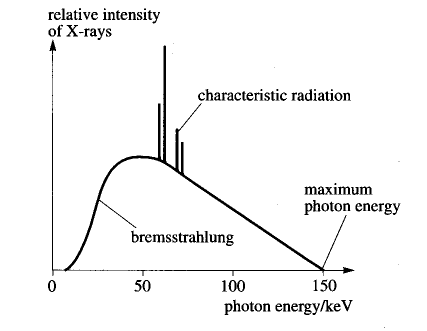
\includegraphics[scale=0.8]{Bremsstrahlung.jpg}
\caption{Shows an Example X-ray emission spectrum from an X-ray tube\cite{xrayemissiondiag}[13]. The spikes originate from characteristic emissions of the material of the anode. The maximum photon energy is dependent on the Duane-Hunt Law.}
\label{2}
\end{figure}

\subsubsection{Synchrotron}

A synchrotron takes advantage of the way in which accelerating electrons emit EM waves. The main principle of the synchrotron is to accelerate high energy electrons around a circular path which is aligned with a series of dipole magnets. As the electrons move along this path, they emit high intensity X-rays along beam lines which are received by sets of detectors on the outer circumference of the path.

\begin{figure}[h!]
\centering
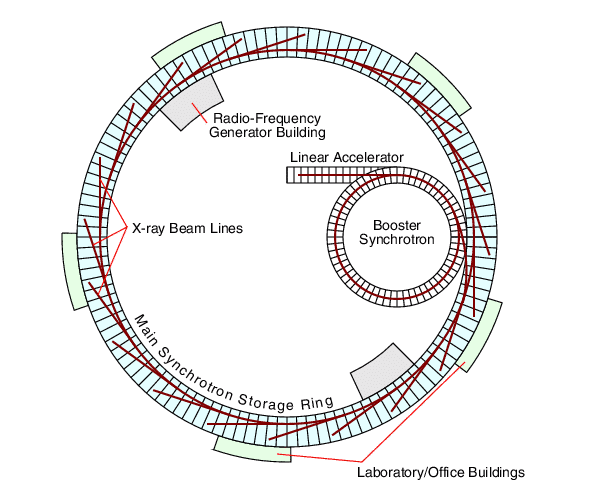
\includegraphics[scale=0.6]{Synchrotron.jpg}
\caption{Shows a schamtic for a simple synchrotron setup \cite{synchrotrondiag}[1].}
\label{2}
\end{figure}

Protein crystals are only weakly diffracting so a high intensity of X-rays is required for crystallisation procedures. Synchrotron X-rays are high intensity, collimated and generally wavelength adjustable and can generate high quality images in a much shorter time frame than X-ray tube methods. For many X-ray imaging techniques, beams with high brightness are required to achieve sufficient spatial resolutions, such beams can be easily generated at synchrotron facilities however access to these facilities can be limited. More innovative methods such as laser-produced plasmas (LPP) offer a means of high intensity X-ray generation and are an alternative to synchrotron x-rays, as in laboratory technique.*

\subsubsection{X-ray Crystallography}

X-ray crystallography is a method by which the structure of a crystalline substance can be revealed. The general basis of the technique is to shine a beam of X-rays, generally produced from some form of a synchrotron, at the desired crystal, the X-rays then diffract off of layers in the crystal. Measuring the angles and intensities of these diffracted beams is used to produce a 3D map of the electron density in the crystal, from which the positions of the atoms in the crystal can be inferred by means of a Fourier transform. 
\begin{figure}[h!]
\centering
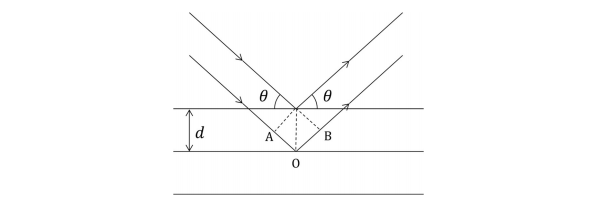
\includegraphics[scale=0.8]{Braag's Law.jpg}
\caption{Shows setup for Braag's law with incident X-ray reflected off of two layers in a crystal \cite{braagslaw}[8].}
\label{2}
\end{figure}

In the context of structural biology, the first X-ray diffraction image of a biological molecule, crystalline pepsin was recorded in 1934 by Bernal and Dorothy Crowfoot. While some proteins naturally exhibit a crystalline structure, more often than not the diffraction of X-rays off of single biological molecules produces only very faint signals, consequently, the samples are generally first crystallised by protein crystallisation methods. A research team led by Zihe Rao et al \cite{virusstructure}[6] at ShanghaiTech University determined the structure of the virus’s main protease using X-ray crystallography at the Shanghai Synchrotron Radiation Facility. Some draw backs of using X-ray crystallography is that the sample needs to first be crystallised. For some bio-molecules, the crystallisation process can prove to be difficult or unfeasible making crystallography methods less appealing when investigating particular samples. 

\subsubsection{Absorption-contrast Imaging}

As X-rays pass through a material they can be absorbed leading to a decrease in the incident beams intensity. This intensity falls according to the Beer-Lambert Law:

$$I(x) = I_0 e^{-\mu z}$$

where $z$ is the materials thickness, $I_0$ is the incident beam intensity and $\mu$ is the attenuation coefficient. When the sample is more complex with many constituent sub-materials (such as a bio-molecule) the attenuation coefficient is considered as non-uniform and the intensity fall follows: 

$$I(x) = I_0 e^{-\int_{0}^{l}\mu (z) dz}$$


where $l$ is the path length of the X-ray beam through material and $\mu(z)$ is the non-linear attenuation coefficient. X-ray absorption-contrast techniques (ACI) examine the attenuation of X-rays as they pass through a sample, the differences in intensity are then used to better understand the sample. Soft X-ray tomographic (SXT) microscopes operate in the water window ($E \sim 285-535 eV$ [13]) and are commonly used in laboratories for imaging bio-molecules which register characteristic spikes between the carbon and oxygen absorption edges  ($\lambda \sim 4.4-2.3$ nm [13]) due to the high carbon content of the organic samples. Newer variations of these methods such as Cryo-SXT can achieve spatial resolutions to the order of 2-3 Å. Paired with cryogenic fluorescence and electron microscopy techniques, Myllys (et al.2018[14]) use Cryo-SXT to study the changes in nuclear architecture and molecular organization of a host chromatin due to herpes simplex virus type 1.

Other absorption-contrast methods include chest radiography, which is commonly used for diagnosis of lung problems such as pneumonia and lung cancer. A projection radio-graph of the chest of the patient is produced by the detection of the attenuated beams on a flat panel detector plate opposite to the patient which are then used in the diagnosis process.  
Joanne Cleverley (et al.2020[4]) goes into detail on how changes on a radio-graph can indicate the presence of Covid-19 pneumonia and discusses the significance of the different features on a radio-graph of a Covid-19 patient. Boran Sekeroglu et al \cite{neuralnetwork} make use of Machine Learning (ML) by using a series convolutional neural networks in the detection of the virus through a set of limited image based data of chest X-rays of Covid-19 patients, yielding a 98.50 percent mean accuracy using the VGG19 pretrained network. Other literature on the use of ML by Tej Bahadur Chandra (et al.2020[5]) present an automatic covid screening system (ACoS), emphasising the importance automatic detection as opposed to slow manual diagnosis due to limited availability of experts. These automatic systems however, require further work and improved reliability for clinical approval.

\subsubsection{Phase-contrast Imaging}

While traditional X-ray imaging methods such as radiography are used for observing the attenuation of the X-rays, Phase-contrast X-ray imaging (PCI) instead examine changes in the phase of the beams as a method of mapping the samples structure. As the X-ray wave-front passes through the substance, it is altered according to the complex refractive index of the sample given by:

$$ n = 1 - \delta +i\beta$$

the imaginary component of which, $\beta$, known as the attenuation index, is related to the absorption coefficient by $\mu = \frac{4\pi \beta}{\lambda}$ where $\lambda$ is the wavelength of the x-ray. The attenuation index determines the rate at which the intensity of the beam 'decays' as it passes through the material. Conversely, the real component $\delta$ dictates the phase of the incoming wave, when the change in real part of the refractive index between two mediums is high, this term dominates and results in an amplitude shift. Procedures which use PCI generally also use ACI to some extent, and work to quantitatively achieve values for the two components of the refractive indices of the bio-molecular components. 
\\
\\
\textit{Propagation Based}
\\
\\
Together with known values for the densities and refractive indices of the constituent organelles of the bio-molecular sample, obtained from previous tests (Cryo-EM), comparisons can be made with the calculated refractive indices to calculate the likely contrast as a function of the energy of the beam[15].


\subsubsection{Cryo-Electron Microscopy}
In cases where the crystallisation of the protein is too difficult or direct images of the viral structure are required it is often more advantageous to use the Cryo-Electron Microscopy (Cyro-EM) technique. Cryo-EM is split into three sub-techniques: electron crystallography, electron tomography and single particle cryo-EM. All three techniques follow the general mechanism of the scattering of electrons off of a the prepared cryogenic sample. An aqueous solution of the biomolecule to be investigated is applied to a thin layered grid which is flash frozen in liquid ethane, the instant freezing of the sample ensures that the water molecules do not crystallize and the sample is formed as an amorphous solid. This vitrified sample is then imaged on an electron microscope. The electron beam which is scattered off of the sample is created in an electron gun in the microscope whereby the heating of the cathode in the gun results in thermionic emission of electrons which are accelerated toward an anode. There is typically an aperture in the anode allowing a collimated beam of electrons to pass through and scatter off of the sample. The signals of the scattered electrons are picked up by a detector and transformed into enhanced images which are then converted to 3D maps of the sample via signal processing and Fourier transforms.
\\
\\
Due to the long wavelengths of emission electrons, electron microscopy techniques can produces images with resolutions of 1Å to 2Å, which is a much higher resolution than what can be obtained from light microscopes which have maximum resolutions of about 200nm. Due to the high impurity tolerance, small sample requirement (approximately 3$\mu$L[12] ) and no need for protein crystallisation, it can be used on demand when viral structure data is required urgently for the characterisation of new strains of the virus and vaccine design. However, due to the high levels of noise associated with using low electron doses to reduce radiation damage, the resolution of images obtained via this method are still lower than that of x-ray crystallography with highest resolutions on the order of about 0.5Å[11].  

Refferences:
\begin{itemize}
    \item [1] http://pd.chem.ucl.ac.uk/pdnn/inst2/work.htm
    \item [2] https://journals.sagepub.com/doi/10.1177/2472630320958376
    \item [3] https://www.medrxiv.org/content/10.1101/2020.10.13.20212035v3
    \item [4] https://www.bmj.com/content/370/bmj.m2426
    \item [5] https://www.ncbi.nlm.nih.gov/pmc/articles/PMC7448820/
    \item [6] https://www.nature.com/articles/s41586-020-2223-y
    \item [7] https://www.orau.org/ptp/collection/xraytubescoolidge/coolidgeinformation.htm
    \item [8] PHAS0041 Lecture notes - Diffraction and reciprocal space 
    \item [9] https://www.tandfonline.com/doi/abs/10.1080/08940888908261212?journalCode=gsrn20
    \item [10]  https://www.sciencedirect.com/science/article/abs/pii/0969806X93E0005P
    \item [11] https://scripts.iucr.org/cgi-bin/paper?S1744309110052607 resolution of x-ray crystallography
    \item [12] https://www.frontiersin.org/articles/10.3389/fmicb.2018.03255/full
    \item [13] http://physicsopenlab.org/2017/08/02/bremsstrahlung-radiation/
\end{itemize}

	\chapter{Spread}
		\section{Containment}
			\subsection{Surface and Air Inactivation}
				

Since the start of the pandemic, the extremely high transmissibility of SARS-CoV-2 has forced scientists to further explore and test all the possible ways of disinfecting frequently touched surfaces, air and water. While mask wearing, good personal hygiene and national lockdowns undoubtedly help reduce transmission, large scale disinfection techniques are still needed. We most often see chemical disinfectants being used worldwide, but Physics has also joined the fight against SARS-CoV-2. 

\subsubsection{UV Light}

The aim of this review is to support the large scale implementation of UV disinfection techniques, more specifically far UV-C (222nm) by grouping together results from various experiments that demonstrate the efficacy of far UV-C in deactivating SARS-CoV-2, as well as its fast, scalable and affordable deployment. We will first show the effectiveness of far UV-C in deactivating other coronaviruses, serving as a testament to the fact that, although scientists are only starting to publish SARS-CoV-2 related experiments, evidence always pointed in favour of this disinfection technique. Then, we will explore the recently documented effectiveness of far UV-C against SARS-CoV-2 specifically, and lastly how it can be implemented in everyday environments. 

UV light is electromagnetic radiation that has wavelength ranging from 10nm to 400nm, and mostly familiar to us as part of the radiation spectrum of the Sun. There are 3 main types of UV radiation: UV-C (100-280nm), UV-B (280-315nm) and UV-A (315-400nm). It is the UV-C type that possesses germicidal properties, first discovered in 1878 against bacteria, and later in 1960 its effect on DNA was found.
Generally speaking, UV disinfection works by acting directly on the virus’ DNA, by breaking the hydrogen bonds and creating thymine dimers (strong covalent bonds between 2 thymine bases), rendering the virus ultimately unable to replicate, thus inactivating it \cite{critical}. Since viruses do not have enzymes, they cannot repair this DNA damage. SARS-CoV-2 is actually a single stranded RNA virus, so instead of creating thymine dimers, UV light creates uracil dimers, but the end result is the same. 
In a RNA molecule, uracil and adenine are bonded via 2 hydrogen bonds. The strongest of these two is the O-H bond, with a bond energy of 459 kJ/mol \cite{chem}. We can convert to Joules by dividing by Avogadro’s number, taken as 6.0221023mol-1. We then use the equation for the energy of a photon: 
$$E=hf=\frac{hc}{\lambda} \iff \lambda =  \frac{hc}{E}$$

to find the wavelength of radiation needed to break that bond:

$$\frac{6.63 \times 10^{-34} \times 3 \times 10^{8}}{\frac{495 \times 10^{3}}{6.022 \times 10^{23}}} = 261 \textrm{nm}$$

which is indeed in the UV-C range.

Buonanno et al. \cite{far uvc effectively} explain that while UV-C (254nm) radiation has been the most commonly used type, it can be a hazard to skin and eyes. However, far UV-C (222nm) light poses significantly less risk to eyes and skin while retaining promising germicidal potential \cite{far uvc effectively} \cite{phys} \cite{safety}. Using 222nm UV light, it is possible to achieve more than 99.99\% reduction of virus in air and on surfaces in a reasonable amount of time in laboratory conditions. Two airborne human coronaviruses exposed in aerosol droplets of sizes similar to those generated during sneezing and coughing \cite{droplets}, alpha HCoV-229E and beta HCoV-OC43, were exposed to different doses of 222nm UV light: 0.5, 1, 1.5 and 2$mJ/cm^2$. After exposure to a dose of 2 $mJ/cm^2$, fractional survival was between 0.001 and 0.0001 for HCoV-229E, and between 0.0001 and 0.00001 for HCoV-OC43 (values are reported as mean ± SEM from multiple experiments). As all coronaviruses have similar size, it would not be unreasonable to assume that similar inactivation results would be obtained if tested on SARS-CoV-2, and the new data does support this hypothesis. These results could be used to devise disinfection measures in a proactive way, in anticipation. Indeed, implementation strategies can be devised as soon as an outbreak is detected, by tuning the UV emitting devices to the correct wavelengths. This is an important note, because different organisms have different susceptibilities to UV radiation \cite{critical}.

Now, we look at the efficacy of 222nm UV light in deactivating SARS-CoV-2 specifically. Firstly, Kitagawa et al obtained 99.7\% reduction of SARS-CoV-2 after exposure to $3mJ/cm^2$ of 222 nm UVC light ($0.1mW/cm^2$ for 30 seconds) in laboratory conditions \cite{kitagawa}. 
Secondly, the first coupled radiation transport and fluid dynamics simulator, based on the Boltzmann Transport and Navier–Stokes equations, was performed by Andrew G. Buchan, Liang Yang and Kirk D. Atkinson \cite{room}. Their model simulated an infected person lying on a bed in a 3m x 3m room used to represent a hospital room or similar. In addition to a ventilation unit, a 222nm UV-C lamp was present. The team reported that with the ventilation unit set to “high” (Air Change per Hour of 8) and with the UV lamp switched OFF, viral removal through ventilation begins 45 seconds after the person exhales once, and concentrations are reduced by 90\% and 99\% in approximately 12 and 24 minutes respectively. With the ventilation set to “low” (ACH of 0.8) and the lamp switched ON, very similar viral reduction was achieved. However, with both ventilation set to “high” and the lamp switched ON, viral reduction by 90\% and 99\% occurred in 6 and 11.5 minutes respectively, which is less than half the time needed compared to the first setting. These results are a testimony that proper ventilation mixed with 222nm UV radiation achieves significant air disinfection results. In addition, this setup can be extended to other similar settings, in elevators for example, where high turnover of people occurs and which experience down times (when nobody is present). Ventilation, coupled with higher intensity exposure of the elevator to 222nm UV, could greatly reduce viral presence in minutes and reassure the population that tight environments can be made safe. Other examples include classrooms: high ventilation during class time, high ventilation and 222nm UV lamp between successive classes or at regular intervals; public toilets, changing rooms, public transports such as buses. With these results in mind, it could be useful to devise implementation strategies including UV disinfection, on top of current measures, especially to enable schools to safely reopen which has been the subject of much debate. Schools can be opened, on condition that extra measures are in place to strongly reduce (the majoritarily asymptomatic) transmission between children who in turn transmit to their household. Moreover, data from the Office for National Statistics from February 2021 show that people working in teaching professions are at 4th highest risk among 25 professions. It is central to children’s social and intellectual development that schools reopen, but this must not be rushed. These results, mixed with a large collection of data regarding the correlation between open schools and a rising number of cases, show that increased ventilation, preferably coupled with 222nm UV-C, would make schools significantly safer.
 
However, it is to note that, while tests have been conducted regarding exposure limit to 222nm UV light on mouse and human tissues, large scale and long term exposure experiments have not been done yet. The tissue tests do not reveal any evidence of potential damage that arises when human tissue is exposed to 254nm UV light, but it is possibly too early to expose people to even 222nm UV until concrete results are published. Furthermore, its effects on clothing, cosmetics and plastics has not been fully studied. That being said, the impact of implementing indirect UV disinfection (whether inside ventilation units or when rooms are clear) is nonetheless substantial, and should be considered especially regarding schools, hospitals, gyms, changing rooms. 

Exploring commercial applications can be a bit more difficult since the extent of the damage caused by 222nm UV light to humans has not been fully explored yet. However, it is still very possible to make indoor environments significantly safer. As previously stated, ventilation already plays a major role in making indoor environments less prone to transmission, and even more so when coupled with UV radiation. Indeed, ventilation units can be fitted with a radiation chamber and HEPA filters just before the air outlet, so the air is much cleaner as it re-enters the room. For larger rooms, a UV light source can be placed in the middle when not in use. The room will be disinfected in less than an hour. Secondly, mobile UV air purifiers are another great application. These machines create clean air flow and can be especially useful in care homes and schools to name a few examples. As for grocery stores, a few machines have been devised to disinfect the frequently touched shopping baskets and trolleys. These machines look like big airport scanners: on one side the customer leaves the basket to be disinfected, on the other side a new customer picks up a clean one. This will help reassure the public about their shopping and help inactivate the virus.

In conclusion, our literature review has helped explore quantitatively the germicidal effect of UV light (222nm UV specifically). Experiments have been conducted for decades to understand the effect of UV-C radiation on viruses. Knowing the disinfection potential of UV light on a family of viruses can help us proactively implement the required UV wavelength to prevent spread. This is because viruses from the same family have similar size and genomic structure, so their genetic material is damaged in the same way. Furthermore, it is important to note that different families of viruses and bacteria have different UV susceptibilities \cite{critical}. This also serves as a warning, since many are taking advantage of the pandemic to sell their products, as it is meaningless to say that a UV light source kills 99.9\% of all viruses and bacteria. 
These findings also do not condone complacency. They help make indoor environments safer, but are not to be taken as a guaranteed replacement to PPE and good hygiene habits. Additionally, these results help support the fact that schools and care homes can, and should, be made safer beyond the usual measures. At the very least, increased ventilation should be implemented in every indoor environment. 
In the near future, it would be interesting to conduct experiments that fully and safely establish the effect of far-UVC (222nm) radiation on human eyes and skin. Furthermore, another area where further experimentation is needed is in combining different wavelengths of UV in LEDs (UVC + UVB for example). This method was tested on E.coli and MS2 virus by Song et al., and the team reported additive inactivation effects \cite{additive}. 



			\subsection{Masks}
			\subsection{Social Distancing}
			
Social distancing has been at the heart of the response against the extremely transmissible SARS-CoV-2. This means staying further apart from others in much smaller groups. The extreme-case example is the lockdown, which has proven to be effective all around the world in reducing cases and deaths \cite{highly inf countries} \cite{phone data} but at the detriment of the economy. While the effectiveness of general social distancing is hard to question in theory, because if you distance yourself you are much less likely to transmit or receive viral particles, there has been some debate about the minimum distance requirements to significantly reduce the risk of transmission. A possible explanation is the complexity of the fluid dynamics involved in particle spread, in addition to all the possible external factors that can affect the flow of viral particles in air such as ventilation, viral load, type of activity (talking, singing, sneezing, coughing). Indeed, complex aerosol based computational models and simulations are needed to help capture the full picture and mechanisms of how transmission takes place, whether indoors or outdoors.
That being said, we here employ a very simple particle trajectory model to familiarise ourselves with the numbers linked with cough and sneeze particles’ trajectories. This does not capture the full details of aerosol transmission, but it can help give an idea of the social distancing needed to help prevent transmission. More detailed, fluid dynamics-based models are used in the Simulations part of the project. 

If we ignore friction, a body thrown upwards follows a parabolic trajectory:

\begin{figure}[h!]
    \centering
    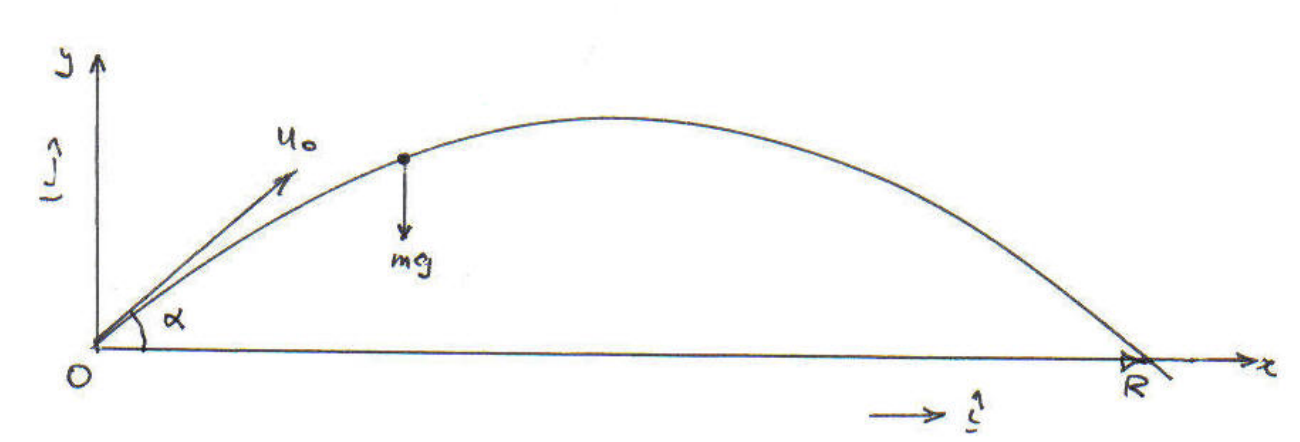
\includegraphics[width=.8\textwidth,clip]{Parabolic trajectory.png}
    \caption{An object's parabolic trajectory on the Earth's surface}
    
\end{figure}

We can use this simple model to predict the trajectory followed by particles emitted when a person coughs or sneezes. This will help give indication about how far others must be to reduce possible transmission. 

We make the following assumptions:
\begin{itemize}
    \item A person’s mouth/nose is at a height of $h=1.8m$ above the ground.
    \item Coughing and sneezing projects particles at $10 m/s$ and $20 m/s$ respectively \cite{distribution droplets}.
    \item Acceleration due to gravity is $g=9.81 m/s^2$.
    \item Coughing projects particles directly forward perpendicularly to the vertical, so angle $\alpha=0$.
    \item No obstruction in the path of the particle's trajectory.
\end{itemize}


We first derive the equations that describe the particle’s trajectory.

The only force acting on the particle is its weight, of magnitude $p=mg$ pointing downwards. From Newton’s Second Law, and splitting into $x$ (positive to the right) and $y$ (positive upwards) directions:
$$
F_x=ma_x=0
$$
$$
F_y=ma_y=-mg
$$
giving
$$
a_x=0
$$
$$
a_y=-g.
$$
But $\textbf{a}=\frac{d\textbf{v}}{dt}$, so
$$
v_x(t)=C_1
$$
$$
v_y(t)=-gt+C_2.
$$
At time $t=0$, using trigonometry, we find 
$$
v_x(0)=v_0cos(\alpha)
$$
$$
v_y(0)=v_Osin(\alpha)
$$
to get 
$$
v_x(t)=v_0cos(\alpha)
$$
$$
v_y(t)=-gt+v_0sin(\alpha).
$$
Then, position vector \textbf{r} is related to velocity by $\textbf{v}=\frac{d\textbf{r}}{dt}$, so
$$
x(t)=v_0cos(\alpha)t+C_3
$$
$$
y(t)=-\frac{1}{2}gt^2+v_0sin(\alpha)t+C_4.
$$
At time $t=0$,
$$
x(0)=0
$$
$$
y(0)=h,
$$
so
$$
x(t)=v_0cos(\alpha)t
$$
$$
y(t)=-\frac{1}{2}gt^2+v_0sin(\alpha)t+h.
$$
We can rewrite the equation for $x(t)$ as $t=\frac{x}{v_0cos(\alpha)}$, which we substitute into the equation for $y(t)$ to finally get
$$
y(x)=-\frac{g}{2(v_0cos(\alpha))^2}x^2+tan(\alpha)x+h.
$$
Since $\alpha=0$, the equation describing a cough or sneeze particle is
$$
y(x)=-\frac{g}{2v_0^2}x^2+h.
$$
The range, which is how far away the particle hits the ground, can be calculated by solving the equation: 
$$
y(x)=0
$$
which has (positive) solution
$$
x_{max}=v_0\sqrt{\frac{2h}{g}}.
$$
As can be seen from this formula, the bigger the initial speed, the further away viral particle can go such as for sneeze particles.

\begin{figure}[h!]
    \centering
    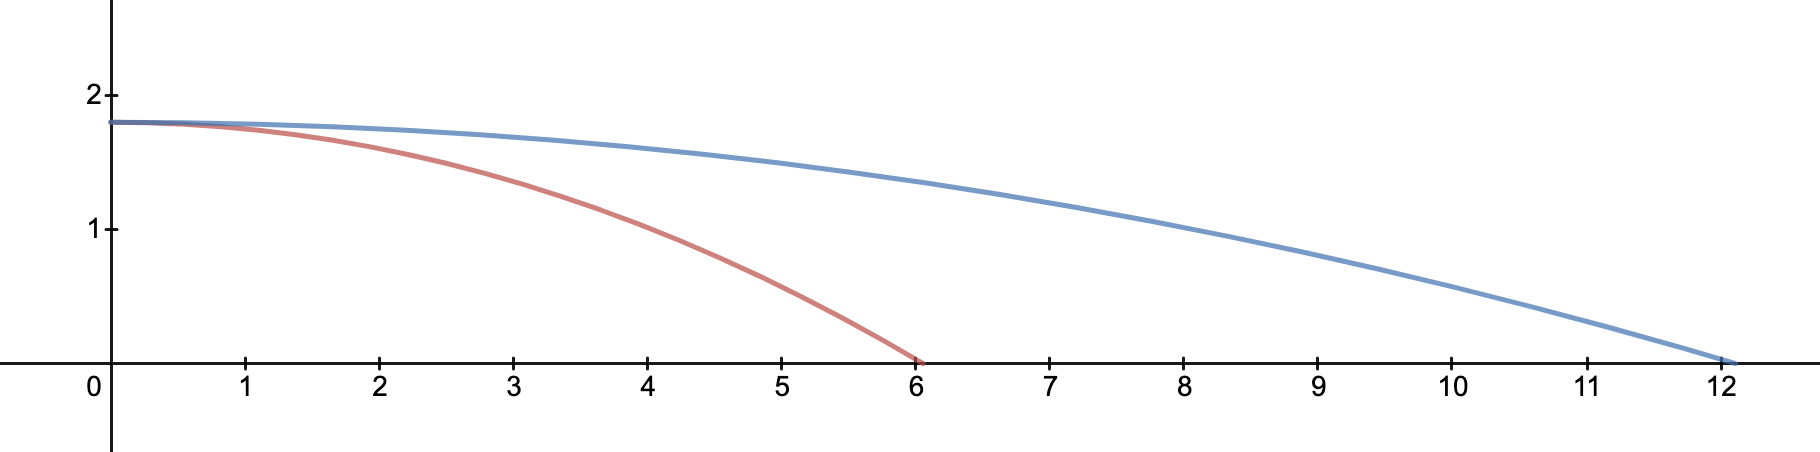
\includegraphics[width=.8\textwidth,clip]{Cough and sneeze trajectory.png}
    \caption{Trajectory of cough (orange) or sneeze (blue) particle from a 1.8m tall person}
    
\end{figure}

We see that from the trajectory of a cough particle, standing 2 meters away is the minimum.  It is 3 meters away and beyond that the drop-off is much more significant and it is likely that transmission would be reduced. 
For a sneeze particle, it goes twice as far so distances should be greater.

That being said, firstly there might be situations where social distancing beyond 2 or 3 meters is not possible. Furthermore, in practice, there are obvious things that can be done to eliminate the risk of transmission, such as using a tissue to cough or sneeze into, and then discarding it. This simple gesture should be done even outside of the context of a pandemic.

\textbf{Wind}

We now add wind to see how it affects the trajectory. Wind speed will be denoted as $v_{wind}$, being positive for left to right wind, and negative for right to left wind.

The new equation of motion is 
$$
y_{wind}(x)=-\frac{g}{2(v_0cos(\alpha)+v_{wind})^2}x^2+\frac{v_0sin(\alpha)}{v_0cos(\alpha)+v_{wind}}x+h.
$$
But, since $\alpha=0$, the equation of motion becomes
$$
y_{wind}(x)=-\frac{g}{2(v_0+v_{wind})^2}x^2+h
$$
and the new range is
$$
x_{max}_{,wind}=(v_0+v_{wind})\sqrt{\frac{2h}{g}}.

We can now plot the wind-adjusted trajectories to compare them with the original path.

\begin{figure}[h!]
    \centering
    \includegraphics[width=.8\textwidth,clip]{Cough wind trajectory.png}
    \caption{ Cough particle trajectory with wind going from left to right at 4m/s (blue), wind going from right to left at 4m/s (orange), normal trajectory in absence of wind (green). Vertical lines represent a person standing different distances away}
    
\end{figure}

\begin{figure}[h!]
    \centering
    \includegraphics[width=.8\textwidth,clip]{Sneeze wind trajectory.png}
    \caption{Sneeze particle trajectory with wind going from left to right at 4m/s (blue), wind going from right to left at 4m/s (orange), normal trajectory in absence of wind (green). Vertical lines represent a person standing different distances away}
    
\end{figure}

By adding wind from right to left (negative) and left to right (positive), we see that the particle’s range is decreased and increased respectively.  
In reality, cough and sneeze particles follow much more complex trajectories that necessitate computational fluid dynamics and other complex simulation tools to be fully described, which are explored in detail in the Simulations section. This does, however, give an indication of how pertinent the 2m social distancing rules are. Once again, wherever possible, 2 meter distancing should be the minimum. It has been shown several times that it helps reduce transmission.

			
			
			
			\subsection{Filtration}
The WHO reports that the primary transmission mode of COVID-19 is through droplet transmission during close contact between people \cite{filt1}. Droplets are defined as being 5 – 10 µm in diameter, and they are produced by the thousands \cite{filt2} when talking for a short time, sneezing and coughing. These are naturally removed from the air in a matter of seconds and travel no further than a few metres, forming the basis for the ‘2 metre rule’ for social distancing in the UK. However, recent evidence also suggests that airborne particles smaller than droplets ($<$5 µm), known as aerosols, can keep the virus suspended in air for much longer and cause ‘airborne transmission’, which does not require close contact. Viable aerosols have been found in large numbers up to three hours after being produced \cite{filt3}, and in one study, a small amount of COVID-19 RNA was identified by polymerase chain reaction test in an aerosol 16 hours after it had been produced \cite{filt4}. The threat of COVID-19 aerosols appears to be an important safety consideration, particularly indoors where there is less movement of air. This section will expose some of the physics of the air filtration technology used to protect against airborne transmission.

A common classification of air filter is ‘high efficiency particulate arrestant’ (HEPA), which in the EU consists of a range of classes centred around an average particle removal efficiency of greater than 99.95\% in a standardised test \cite{filt5}. One important control in the test is that the mean diameter of the aerosols corresponds to the ‘most penetrating particle’ (MPP) through the device, which has a filter-dependent diameter that can be calculated once the filtration mechanisms are understood. For most HEPA filters, the MPP is about 0.3 µm. This means that for particles sizes both greater and smaller than the MPP, the air filter will be even more effective, as a result of its mechanisms of removal, which are the same as for masks [see section: Masks].

An important study by Miller-Leiden et al. (1996) \cite{filt6} investigated how useful air filters were when used with ventilation at reducing the concentration of test aerosols in a room in response to Tuberculosis transmission, testing many scenarios. Unsurprisingly, it was found that HEPA filters reduce the concentration of aerosols more effectively when they perform more ‘air changes per hour’, which is a measurement of the volume of air filtered per unit time. However, the authors concluded that the most effective use of air filters was to use them in conjunction with ventilation, and to have them positioned close to the source of aerosols.
			
			
		\section{Eradication}
		
The CDC defines eradication as a “permanent reduction to zero of the worldwide incidence of infection caused by a specific agent as a result of deliberate efforts; intervention measures are no longer needed”. One of the best ways to achieve this is through a successful vaccine rollout in the affected areas and beyond to immunise the whole population. Since the outbreak of SARS-CoV-2 was announced as an pandemic in March 2020, enormous human, scientific and financial efforts of collaboration have been made to quickly devise vaccines. As more and more companies publish their data about successful trials, we get closer to defeating this microscopic, biological enemy, but the problem of vaccine storage remains a threat to the rollout. Indeed, vaccines have very clear thermostability guidelines that govern their immuno-integrity and potency. This means that they must be stored and kept within a range of cold temperatures even during transport, which puts extra stress and strain on the cold chain. According to the WHO, “the cold chain consists of a series of links that are designed to keep vaccines within WHO recommended temperature ranges, from the point of manufacture to the point of administration”. In laboratory facilities, specialised freezers and refrigerators are used to safely store vaccines, but during transport, temperature monitoring is even more crucial. This section focuses on the reason why vaccines need to be kept extremely cold, and the physics behind how these temperatures are achieved.
		
			\subsection{Vaccine Storage}

\textbf{Why do vaccines need to be stored in cold temperatures?}

At all times, the contents of the vaccine must be kept intact by stopping any naturally occurring processes or interactions of the different molecules. Indeed, some of the distributed COVID-19 vaccines are based on mRNA technology (Pfizer and Moderna for example). mRNA molecules are extremely fragile. Indeed, “One reason RNA is much less stable than DNA is due to an important difference in the sugars that make up the molecules’ backbones. RNA’s spine is a sugar called ribose, while DNA’s is deoxyribose. The difference: DNA is missing an oxygen molecule. As a result, “DNA can survive for generations, but RNA is much more transient” says Sanjay Mishra, a protein chemist and data scientist at Vanderbilt University Medical Center in Nashville \cite{mrna}. Furthermore, RNA molecules are usually quickly destroyed  by enzymes once they have served their purpose. This short RNA lifetime makes it vital that the vaccine constituents are always in the correct conditions to stay intact, to ensure an effective immune response is generated in the patients. Very cold temperatures help freeze out any possible processes, similar to refrigerating a piece of chocolate to prevent it from melting. 
In addition, temperature must be kept as constant as possible. Fluctuations can lead to crystallisation of some components of the vaccine, breaking the membrane for example.

\textbf{How low does the temperature need to be for the different vaccines?}

The Pfizer vaccine needs to be stored at -70℃. For this, Pfizer has devised special, temperature-controlled containers filled with dry ice to store its vaccines during shipments. It can be stored in a laboratory-grade refrigerator between 2℃ and 8℃, but only for a few days.
The Moderna vaccine’s storage temperature is -20℃, which is achievable with most existing storage equipment in laboratories. It can be stored at 2-8℃ for 2-4 weeks.
Lastly, because of the vaccine technology used, Oxford and AstraZeneca say their vaccine can be safely stored in laboratory-grade refrigerators at 2-8℃.

The stringent storage guidelines do pose extra stress on the cold chain. Significant investments have been made and measures have been taken to ensure proper distribution of these vaccines, given the severity of the situation.

\textbf{How do you get the temperature down to -70℃?}

Dry ice (solid $CO_2$) is the core element in keeping temperatures this low. To make dry ice, $CO_2$ gas is pressurised and cooled into liquid form. Then, the pressure is decreased to let the $CO_2$ expand back into gas form, which rapidly causes a drop in temperature.
$CO_2$ goes from solid phase to gas phase (sublimation) following an increase in temperature at constant atmospheric pressure as seen from the phase diagram. 

\begin{figure}[h!]
    \centering
    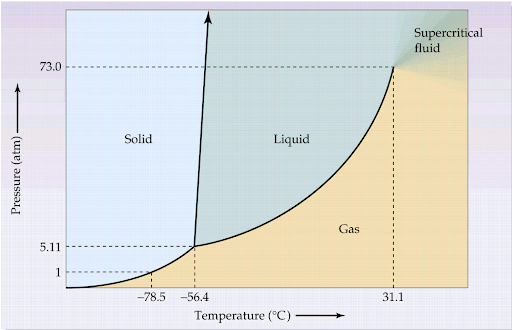
\includegraphics[width=.8\textwidth,clip]{Phase Diagram of CO2.png}
    \caption{Phase diagram of carbon dioxide ($CO_2$)}
    \label{Phase Diagram}
\end{figure}

\textbf{Why does $CO_2$ sublimate?}

This is partly due to the weak intermolecular bonding between $CO_2$ molecules, caused by its geometry. Indeed, a $CO_2$ molecule is a linear, nonpolar molecule, as opposed to, for example, a water molecule that has a triangular geometry and is polar.

Sublimation is an endothermic process that happens below a substance’s triple point (lowest pressure at which liquid phase exists). This isobaric process happens through the absorption of heat (energy) from the surrounding air. This heat gives molecules higher velocity and therefore higher kinetic energy which breaks the inter-molecular bonds found in solid state. The pressure of the triple point of $CO_2$ is 5.11 atm.

There is interesting thermodynamics involved in sublimation. Any substance wants to, and will, configure itself to minimise its Gibbs Free Energy at a given pressure and temperature. Gibbs free energy $G$ is given by
$$G=U+pV-TS=H-TS$$
where $U$ is internal energy, $p$ is pressure, $V$ is volume, $T$ is temperature, $S$ is entropy and $H$ is enthalpy. 

Below is a table summarising how each variable changes depending on the phase.

\begin{figure}[h!]
    \centering
    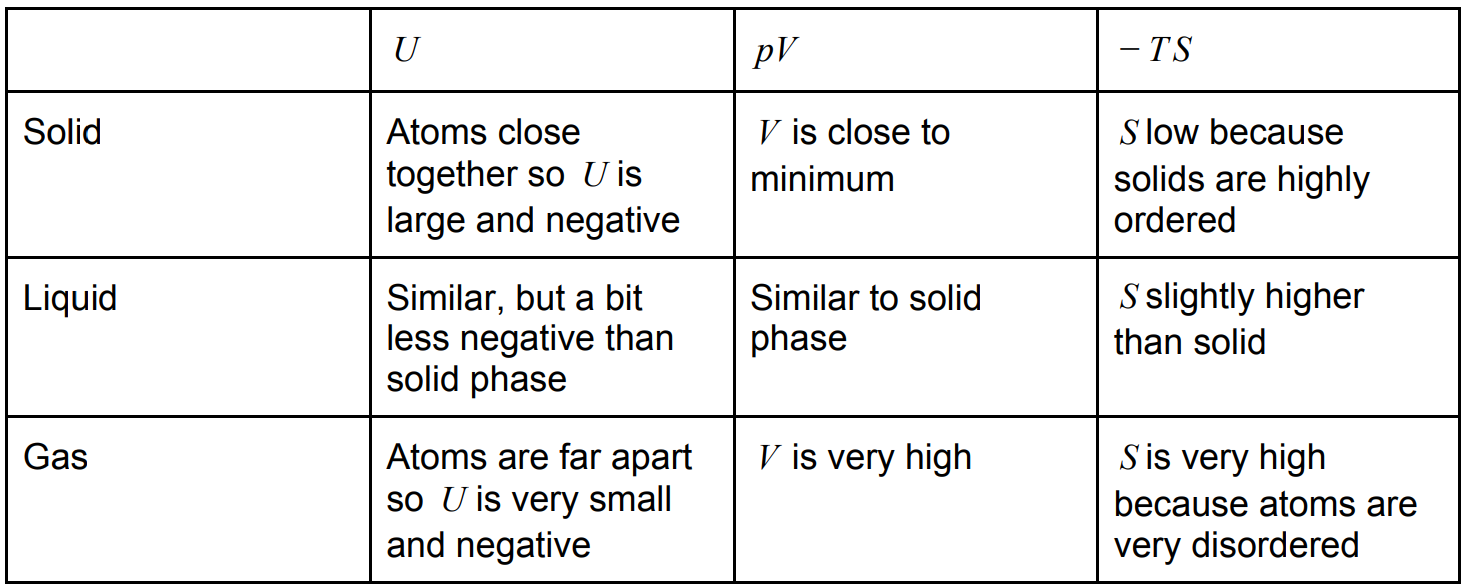
\includegraphics[width=1.1\textwidth,clip]{Gibbs Table.png}
    \caption{Summary of changes in the variables that appear in the gibbs free energy equation}
    \label{Gibbs free energy relations}
\end{figure}

 We can now look at the G vs T graphs at various pressures:
\begin{figure}
    \centering
    \begin{subfigure}{1.0\textwidth}
        \centering
        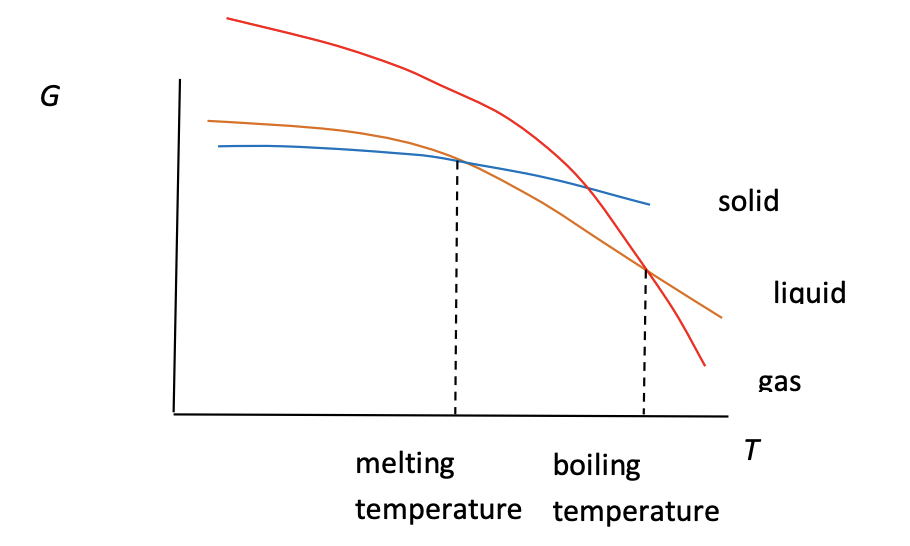
\includegraphics[width=0.7\linewidth]{ptrip.p.pcrit.png}
        \caption{$p_{triple}<p<p_{crit}$}
        \label{fig:sub1}
    \end{subfigure}
    \begin{subfigure}{1.0\textwidth}
        \centering
        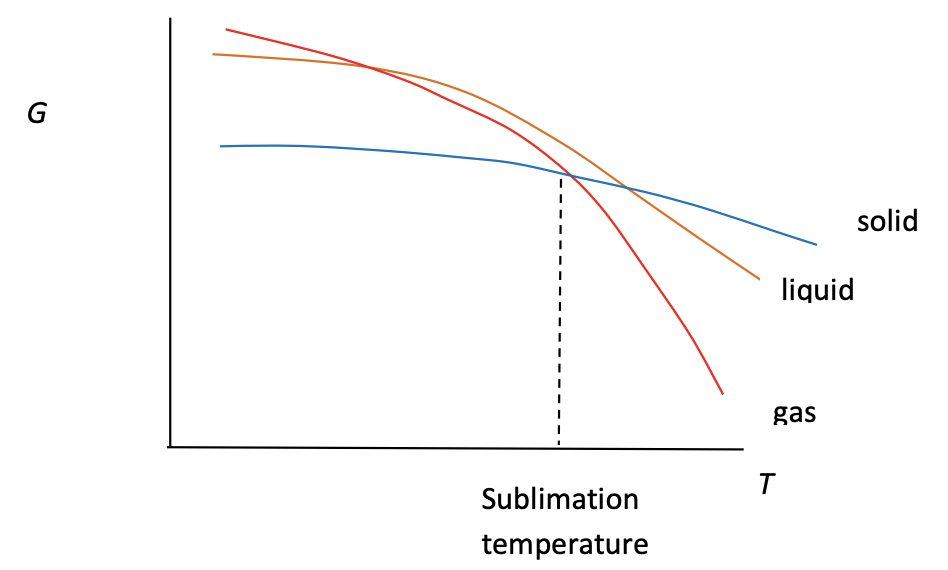
\includegraphics[width=0.7\linewidth]{p.ptriple.png}
        \caption{$p<p_{crit}$}
        \label{fig:sub2}
    \end{subfigure}
\caption{\textbf{G vs T graphs for various pressures}
a) graph of G versus T for a substance in the solid, liquid and gas phases for $p_{triple}<p<p_{crit}$
b) graph of G versus T for a substance in the solid, liquid and gas phases for $p<p_{crit}$
}
\label{fig:test}
\end{figure}

Below the triple point, a solid sublimates (changes from solid to gas without passing through a liquid phase) because after the solid phase, the next phase with lowest Gibbs free energy is the gas phase. The liquid is not the equilibrium state at any temperature.
Also, $$\left(\frac{dG}{dT}\right)_p=-S$$ therefore the slope of the curve is always negative and it is more negative for a gas than for a liquid or solid because the gas has higher entropy.			
Since $CO_2$’s ptripleis 5.11atm, normal atmospheric pressure of 1atm will lead to sublimation of solid $CO_2$ as the temperature increases. 

So by using dry ice in containers, Pfizer says its vaccine can be stored for up to 15 days unopened. According to Pfizer, this storage time can be extended if the containers are re-iced every five days, until the vaccines from that particular shipment have all been administered. This has made dry ice a critical component in storing vaccines during shipment at extremely cold temperatures. In addition, not only is dry ice cold enough to store the Pfizer vaccine, it also does not melt, unlike regular ice, so it does not leave a messy puddle in the container.

For vaccines that can be safely stored between 2℃ and 8℃, they can be stored in laboratory refrigerators. These refrigerators have very precise and accurate temperature monitoring capabilities, to ensure vaccine integrity. Most also have special lining inside to keep the temperature within the 2-8℃ range for 1 or 2 hours in case of a power outage.

\textbf{But how does a refrigerator or freezer work?}

Essentially, a refrigerator extracts heat from the compartment inside and rejects it to the surrounding environment (kitchen or laboratory), cooling the inside. 
It is important to remember the Second Law of Thermodynamics, which states  that heat flows spontaneously from a hot body to a cold body. 
The main components involved in the refrigerator cycle are:
\begin{itemize}
    \item a compressor that does work on the refrigerant gas, plugged into an electrical socket
    \item a coil that runs outside the refrigerator 
    \item an expansion valve
    \item a coil that runs inside the refrigerator.
\end{itemize}

The refrigeration cycle is as follows:

Firstly, the compressor does work on the gas, increasing its pressure and thus its temperature. This is because, for an adiabatic process,
$$TV^{\gamma -1} = C$$
where $\gamma$ and $C$ are constants. So if we consider an initial state with $T_1$ and $V_1$, and a final state $T_2$ and $V_2$, then,
$$T_1V^{\gamma -1}_1 = T_2V^{\gamma -1}_2$$
and therefore
$$\frac{T_1}{T_2} = \left(\frac{V_2}{V_1}\right)^{\gamma - 1}$$
We indeed see that if $V_2 < V_1$, then $T_2 > T_1$.

Secondly, this compressed, hot gas flows through the coil that runs outside the refrigerator, and loses heat to the surrounding, colder air. The gas then condenses to a liquid.

Then, the newly formed liquid goes through the expansion valve, decreasing its pressure and temperature.

This liquid now flows through the coil located inside the refrigerator, inside which the air is hotter than the liquid.

Since the liquid is colder than the air, it absorbs the heat that is inside the refrigerator, reducing the temperature of the compartment. 

Finally, the liquid evaporates into a gas thanks to the absorbed heat, and the cycle restarts.

\begin{figure}[h!]
    \centering
    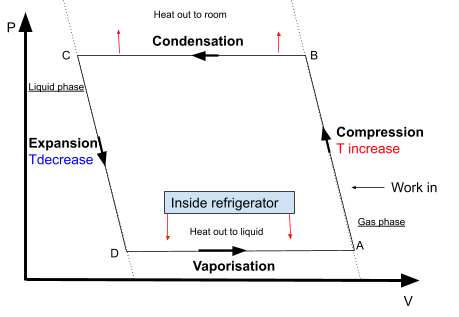
\includegraphics[width=1.1\textwidth,clip]{PV.refrigeration.cycle.png}
    \caption{P-V diagram of refridgeration cycle, starting at a point A}
    \label{Refridgeration Cycle}
\end{figure}

This cycle runs only when needed. When the inside temperature goes over a certain limit, the cycle starts to cool the inside again. When the temperature is back in the desired range, the cycle stops. Refrigerators usually stay between 2℃ and 8℃. If ice builds up inside the refrigerator or freezer, this obstructs the flow of heat from the compartment to the refrigerant. To compensate, more work will be done and energy use will increase by the refrigerator or freezer. This is why regular defrosting is necessary.


		\section{Treatment}
			\subsection{Ventilators}
			
Ventilators are critical for patients suffering from severe COVID-19, when a condition called ‘acute respiratory distress syndrome’ (ADRS) develops, meaning that the alveoli in the lungs are so inflamed that fluid enters the lungs, filling some of the air sacs and causing some alveoli to stick together. Assisted breathing with a ventilator reduces the strain of a patient by using mechanically generated positive air pressure to fill the lungs instead of abdominal muscles. A ‘baseline’ of positive pressure in the lungs can also help to keep the alveoli open and reopen those that are closed due to inflammation fluid leaks.

Ventilators work according to a number of relations that are very familiar to physics. The dynamic system of a pair of lungs on a ventilator is accurately modelled by \cite{vent1}:

\begin{equation}
    P_{rs} = EV + R\dot{V} +k
\end{equation}

where $P_{RS}$ is the pressure in the respiratory system, E is the ‘elasticity’ of the lungs, V is the volume of the lungs, R is the resistance to the airway, $\dot{V}$ is the air flow (the time derivative of the volume) and k is the approximately constant pressure in the lungs after exhalation is complete. This equation resembles a classical equation of motion, and important concepts of ventilator function can be derived from it.

Modern ventilators have advanced settings to control their positive pressure, but here only the pressure mode and volume mode will be considered. This means that an assisted inhalation is characterised by either a maximum pressure being reached in the lungs or a maximum volume of air being detected in the lungs. One assumption that is also made is that the pressure due to the patient’s muscle contractions is negligible. Figure 1 shows the typical phases of a breath on a mechanical ventilator:

\begin{figure}[ht]
\centering
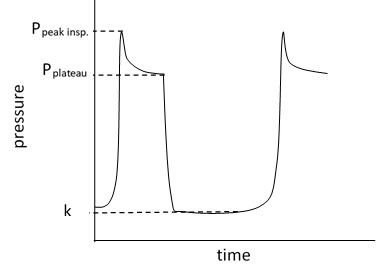
\includegraphics{pressure time graph.jpg}
\caption{Typical graph of pressure against time for a mechanically ventilated patient.}

\end{figure}

Working in the volume mode, the elasticity of the lungs can be calculated. During ventilation, an initial volume of air is rapidly blown into the lungs, and then held there. The pressure will decrease to a constant value, $P_{plateau}$, as the air disperses uniformly until there is no flow. The elasticity is then determined by dividing the overall increase in pressure by the volume of air put into the lungs. The reciprocal of the elasticity is called the static ‘compliance’ of the lungs, C.

\begin{equation}
    E = \frac{P_{plateau}-k}{V} = \frac{1}{C}
\end{equation}

The resistance to air flow R is calculated by measuring the lungs in a dynamic setting. The pressure drop from the peak inspiratory pressure to the plateau while the air is dissipating is measured and divided by the flow of air during this time.

\begin{equation}
    R = \frac{P_{peak\:{}insp.}-P_{plateau}}{\dot{V}}
\end{equation}

The resistance can also be described by the classical Poiseuille’s law \cite{vent2}, which describes how a fluid moves through a long tube under ‘laminar flow’ conditions, where fluid particles are modelled as separated into layers with different velocities. The equation for resistance from Poiseuille’s law is:

\begin{equation}
    R=\frac{8\mu{}L}{\pi{}r^{4}}
\end{equation}

where $\mu{}$ is the fluid viscosity, L is the length of the tube and r is the radius of the tube. This describes the resistance of the lungs well, and can be used to infer problems with the lungs as resistance changes, for example a small decrease in the radius of the airway will cause a much more significant increase in resistance. From this equation it may be expected that the thinnest airways in the lungs provide the most resistance to air flow, but the tubes in the lungs are analogous to electrical resistors. Therefore the larger number of smaller tubes effectively in a parallel resistor configuration reduces their overall contribution, and it is the largest airways which provide the most resistance to airflow \cite{vent3}.

During a patient’s time on a ventilator, compliance and resistance are constantly measured as they can be used to detect the onset of respiratory complication, requiring adjustment of settings. For example, the ADRS that is associated with COVID can cause a decrease in compliance due to the alveoli that are clogged with fluid \cite{vent4}. An increase in the air pressure provided may then be required.

Small studies have been performed on ventilated COVID patients to investigate its effects on lung mechanics so that ventilators can be appropriately set to maximise benefits to patients. There is no clear consensus yet, with some showing effects closely resembling typical ARDS reductions in lung compliance \cite{vent5}, while there have also been suggestions that some COVID patients can progress to an unusually high compliance for ADRS as well \cite{vent6}. However, these high compliance occurrences may be the result of damage done to the lungs by the body’s response to the ventilator itself, and so it has been recommended to pay particular attention to the individual’s needs when it comes to ventilation to alleviate this effect \cite{vent7}.

			
			
			\subsection{In Vivo Inactivation}
			
				\subsubsection{Introduction}
			
				\noindent M. Babincová et al. proposed \cite{resonant} a method for eradicating enveloped viruses using ultrasound based on their highly symmetric structure, such that there exist one or a few isolated resonance frequencies. In the case of many viruses, the symmetry is icosahedral. A similar simplicity may be expected in the vibrational spectra of these viruses to that of the icosahedral buckmisterfullerene molecule, which has $4$ instead of the $60 \times (3 - 6) = 174$ frequencies found in molecules with 60 atoms which do not exhibit this symmetry. \\
			
				\noindent Noting that resonant frequency corresponds to a wavelength of the same order as the object, the frequency for HIV may be estimated using $f=\frac{c}{\lambda}$, where $f$, $c$ and $\lambda$ are the resonant frequency, velocity, and wavelength of the sound, respectively. In the case of HIV, $\lambda \sim 100 \mathrm{nm}$, $c \sim 1000 \mathrm{~ms}^{-1}$, the speed of sound in tissue, therefore $\mathrm{f}=10 \mathrm{GHz}$, a high frequency ultrasound. \\
			
				\noindent L. Ford provided \cite{estimates} more accurate estimates of the normal modes of vibration of nearly spherical virus particles using a liquid drop model and an elastic sphere model. The liquid drop model considers a sphere of radius $a$ filled with a nonviscous liquid with surface tension $\gamma$ and mass density $\rho$. The lowest vibrational mode of this sphere will be a quadrupole mode with frequency $\nu=\frac{1}{\pi} \sqrt{\frac{2 \gamma}{\rho a^{3}}}$ which can be written as $\nu=3.4 \times 10^{8} H z\left(\frac{50 n m}{a}\right)^{\frac{3}{2}}\left(\frac{\rho_{W}}{\rho}\right)^{\frac{1}{2}}\left(\frac{\gamma}{\gamma_{W}}\right)^{\frac{1}{2}}$ where $\rho_{W}=10^{3} k g / m^{3}$ and $\gamma_{W}=0.073 N m$ are the mass density and surface tension for water, respectively. The surface tension and mass density, along with the lowest vibrational frequency derived using this equation for $a=50 n m,$ are given in a table for several liquids. Based on agreement with the elastic sphere model, it is concluded that this frequency is likely to be on the order of a few GHz for particles with a radius on the order of 50nm.
			 
			
				\begin{table}
			 		\centering
					\begin{tabularx}{\textwidth}{|X||c|c|c|}
					\hline \hline Liquid & $\gamma / \gamma_{W}$ & $\rho / \rho_{W}$ & $\nu /\left(10^{8} H z\right)$ \\
					\hline Benzene & 0.397 & 0.88 & 2.3 \\
					Diethylene glycol & 0.62 & 1.12 & 2.5 \\
					Trehalose & 0.95 & 1.63 & 2.6 \\
					Lysine hydrochloride & 0.90 & 1.38 & 2.7 \\
					Arginine hydrochloride & 0.95 & 1.44 & 2.8 \\
					\hline \hline
					\end{tabularx}
					\caption{The mass density, surface tension, and the lowest vibrational frequency predicted for drops of various liquids with a radius of $a=50 \mathrm{nm}$. The data for Benzene and Diethylene glycol are for droplets in air at room temperature, the data for the three proteins for aqueous solutions at $\sim 50^{\circ} \mathrm{C}$.}
				\end{table}
				
			\subsubsection{Vibrational Modes}
			\subsubsection{Raman Spectroscopy}
			\subsubsection{Empirical Work}
						
	\chapter{Simulations}
		\section{Introduction}

\label{sec:intro}    

\subsection{Introduction to computational methods in applied physics}


Applications of computational science in physics is a powerful tool which gives an insight and analysis about a particular physical system being studied. Specifically, the underlying framework based on theories and assumptions governing physical laws enables the possibility to model and formulate realistic simulation of the evolution of a particular system. With the unique advantage of open access to change the parameters and underlying assumptions enables an accurate and reliable comparative study of different scenarios of a particular system. In real-life experimental set-up, there are various constraints which limit the degrees of freedom and this further limits the observation of certain effects in depth and fails to give clarity on the true source of the cause of effect. Additionally, the lack of availability in constructing a perfectly vacuum condition to examine certain high sensitivity processes gives rise in uncertainties which may not be necessarily systematic. 

Alteration parameters of the model allows to accurately observe the particular change in the desired properties of the system. Certain physical properties can be extracted from the model with ease without the introduction of various non-systematic errors resulting from measurement. Modeling idealised scenarios under perfect vacuum conditions without interference of external noise decreases set of uncertainties resulting from interference and as a result, can be used in developing theories to be implemented and tested. Various properties and quantities of the particular system can be extracted and analysed though the change of procedures with the implementation of the appropriate algorithms. Furthermore, complex dynamical systems with high degrees of freedom can be studied and analysed with high accuracy using algorithms.

Particularly, computational physics is essential in handling a set of problems ranging from non-linear systems to chaotic processes. Complex physical processes are often always non-linear at best and can be chaotic. Non-linear processes are used to describe events which have non-linear dependence, altering a certain parameter may not necessarily result in a linear response of the system. Non-linear second order problems and chaotic processes are complex and multiple parameters must be considered simultaneously due to its nature of high degree of freedom. Solving such problems through numerical methods implemented by algorithms can obtain high accuracy solutions. In numerical solution construction, the system of  second order non-linear equations describing the system is classified as a parabolic. The complexity can be further extended to a mix of parabolic, elliptic or hyperbolic partial differential equations (PDE's). To improve accuracy, numerical errors and boundary condition specification must be considered.

Additionally, these highly complex systems have multiple parameters and variables and give rise in difficulty in extracting certain dynamical properties of the system. Dimensionality reduction which  collapses the complex system described by $N$ dimensions to a lower dimension through the implementation of algorithms reduces the complexity of the system with minimal loss of the intrinsic properties of the system. Analytical methods can be used to evaluate the optimal reduction algorithms to the network. The loss of intrinsic proprieties resulting from dimensionality reduction is evaluated by comparing the predicted parameters to the actual response of the system. 


\subsection{Application of computational physics in airborne transmission of virus}

SARS-CoV-2 commonly referred as COVID19 is a viral infectious agent which causes respiratory complications and in some cases lead to mortality. Considering the different pathways of the transmission of the virus, airborne transmission in the context of an indoors environment has had the most significant impact on increasing infection rates. The airborne transmission of the active virus can be classified as aerosol particles, which are a collection of microdroplets ranging in size of order of magnitude of 10 \si{\micro\meter}. It has been observed that both long-range and short-range airborne transmissions are possible which considerably increases the rate of transmission. The high airborne transmission rate of aerosols and the longevity of the survival period of the virus are causing difficulties and delays in containment procedures. As a result, COVID19 has been officially declared a pandemic after just two months of its initial recorded case.

With the imposed weights on modern healthcare systems and effects on economies all over the world, there must be heavy emphasis towards the development of strategies on the eradication of the disease. Current policies and practices must be reconsidered. In this paper, applications of computational physics will be used to analyse various proposed methodologies in tackling the containment of spread of the virus towards the eradication of COVID19.

\section{Monte Carlo Methods}

\subsection{Introduction to Monte Carlo Methods}

Monte Carlo Methods date back to the 18th century initially proposed by a mathematician Georges-Louis Leclerc, Comte de Buffon, to estimate the value of $\pi$ by tossing a needle with length $L$ onto a sheet with plane parallel lines with a separation distance of $d$. Probability occurrence for an event where a needle is tossed at random to land to intersect a line on the sheet has been estimated as $P(x)=\frac{2L}{\pi d}$. Note that the needle is shorter than the distance between parallel lines on the sheet $L<d$. The solution was obtained using integral geometry. A diagram representation of the needles tossed at random is shown in Figure. \ref{Needle}.  With each random toss of a needle represented by an 'event' $N_i$ and each event $N_i$ can be further represented by coordinates $(\theta, x)$. Assuming that there was no $\pi$ variable in the above mention equation, $\pi$ can be estimated by recording the number of events where the needle crosses the line. A graph representation of this procedure is shown in Figure. \ref{pi}. With increasing number of events, the approximation of $\pi$ increases in accuracy. This was the first recorded example of using randomness to solving a deterministic problem. The origin story suggests the versatility of Monte Carlo methods as a framework of predicting the outcome of a certain processes.


\begin{figure}[h!]
    \centering
    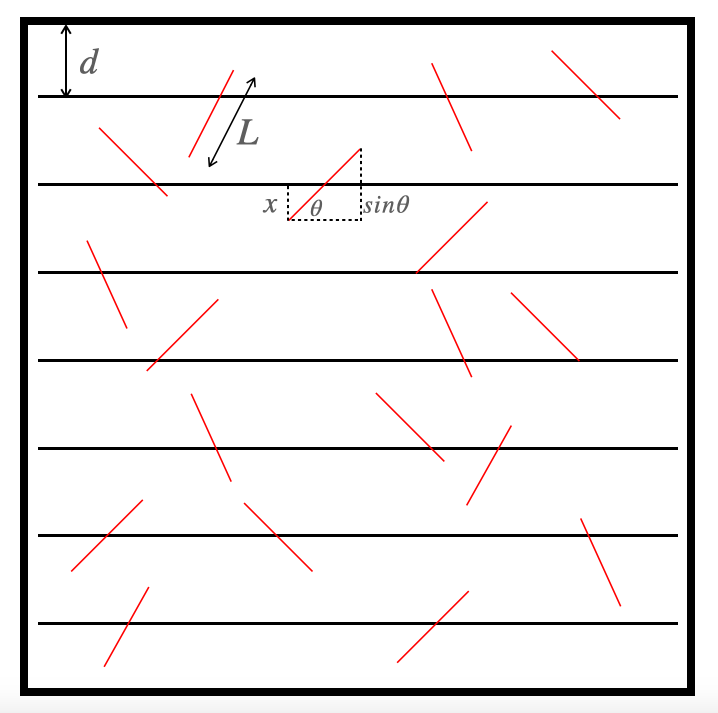
\includegraphics[width=.30\textwidth,clip]{Needle.png}
    \caption{A diagram of needles of length $L$ randomly tossed on a sheet with plane parallel lines, with separation distance $d$, with $L<d$}
    \label{Needle}
\end{figure}



\begin{figure}[h!]
    \centering
    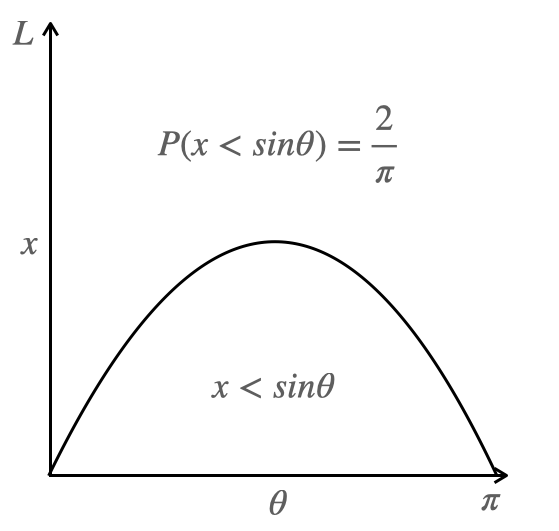
\includegraphics[width=.30\textwidth,clip]{pi.png}
    \caption{The estimated probability distribution of the event where needle intersects the line given the needle is tossed at random, with $L \approx d$}
    \label{pi}
\end{figure}


Monte Carlo Methods are especially useful in simulating the time evolution a complex system with many degrees of freedom. A sequence of probability distributions are used to describe the time evolution of a non-linear systems. The most recent state of the non-linear system depends on the transition probability and is extracted from the random distribution of the current probable states of the system. For systems with high degrees of freedom, many parameters including the available path and the boundary conditions determine the evolution of the system, with each parameter having non-linear effect in its influence towards the output. Multiple simulations must be implemented, considering the most recent state of the system depends on the previous state. Now the time dependence of the system will no longer be a remarking feature, as multiple simulations will minimize the variance of the differences in the output of each simulation. With the averaged final state of the non-linear system will converge to an equilibrium state, or a stationary distribution within a valid range of error. The central limit theorem gives a description of the convergence of the random variables for each simulation.

A large system of particle interactions are classified under the mean-field free particle method. As the size of the system increases with $N$, the number of particles approaching a range of $10^{23}$ particles, necessary measures need to be taken to reduce the system. The reduction measure will be to estimate the system as a macroscopic system, where the dynamics of the system is described through sets of non-linear partial differential equations. The information of this system will be extracted by solving the sets of non-linear PDE's numerically. Considering the size of the system and macroscopic feature, the probabilistic interaction between each particles will no longer factor in, and only long range interactions are considered. As the limit of particles tend to infinity, the discrete description tends to a description of continuous partial differential equations (PDE's).



\subsection{Mathematical framework of Monte Carlo Methods}

 The response of the interactions of the particles will be averaged over multiple individual particle simulations, to obtain the true average $\overline{x}$, with a stationary distribution of $x_i$, and a true finite variance $\sigma_x^2$. To ensure 


Random position generator 

Explain the theories and maths behind the general monte carlo??? 
type of distribution 
type of sampling 
random number generator 
displacements 
mean and variance 


\section{Mathematical Methods in Modeling Disease Spread}



\subsection{Stochastic Diffusion Processes}

Stochastic processes are classified as a subdivision of concepts from statistical mechanics and probability theory. The nature of stochastic processes are probabilistic. They are most useful in describing complex, random chaotic systems. Monte Carlo techniques are described by stochastic processes. Stochastic processes utilise the concept of Markov process. A Markov process is a probabilistic theory of the classical theory of mechanics, characterised as a system independent of memory and time-dependence, the immediate outcome of the system is represented as a probabilistic state. The probability of the transition to the subsequent step $n_i$ dependent on the most previous state $n_{i-1}$, with a conditional probability $P(n_i|n_{i-1})$, where $i$ is the time-step. Markov processes are used in simulations to describe the time evolution of a system approaching an equilibrium state, with initial set boundary conditions.

The diffusion equation is a solution to the stochastic equation describing the motion of random particles. Particularly, Brownian motion gives a classical description of the dynamics of indistinguishable particles. The interactions between the particles are approximated using Newtonian description. For a system of $N$ particles, the evolution of the system can be described by stochastic differential equations (SDE's).

Discrete Lagrangian Stochastic particle model
Link to the actual process of simulation!!!


\subsection{Eulerian particle model}

The particle of aerosol dissipation was modeled using the Euler approach. In the Eulerian framework, the individual particle interaction is not the defining feature, particle interactions are defined as a whole, a collection of particles which form a fluid contained in a defined control volume. The properties of the fluid such as the pressure and velocity are approximated as fields, and can be described in terms of a function of space and time. The continuous dynamical properties of the system are the defining feature rather than the position of individual particles in a specified time-frame. As a result of the features, the Eulerian approach best describes fluids due to their continuous nature. The fundamental laws for equation of motion are modified in this approach. For instance, in the Eulerian approach, the motion of fluid flow is described by "velocity of field" compared to velocity of their individual particles. 

\begin{equation}
    \Vec{V}(x,y,z,t) = u(x,y,z,t)\Vec{i}+ v(x,y,z,t)\Vec{j} + w(x,y,z,t)\Vec{k}
\end{equation}

The velocity vector $\Vec{V}$ has three spatial components $u,v,w$ which are functions of space and time $x,y,z$ and $t$. At some particular point in space $(x,y,z)$ and time $t$ there is a field velocity vector $ \Vec{V}(x,y,z,t) $. 

\subsection{Diffusion Equation}

The aerosol particles undergo the process of diffusion, where the flow of particles transport against the concentration gradient. To reach equilibrium, the flow of particles diffuse from an area of high concentration to low, which can be described as $-D \frac{dN}{dz}$, where $D$ is the diffusion constant. Diffusion process occurs in an open system and is influenced by various parameters including $D$ which depends on the temperature of the system and the medium for which the process will occur in, in this case, air. Since aerosol particles are in gaseous form, it has low concentration of particles per unit volume, as a result, the process is rapid since less particles are required to reach their respective equilibrium position. Due to the continuous nature of this process, the diffusion equation is derived from continuity equation. The continuity equation relates the rate of change of some scalar quantity in some differential control volume to the flow and diffusion process of particles into and out of the system.

The diffusion equation used to describe the aerosol flow is a non-linear ODE of the form:

\begin{equation}
    \frac{\partial c}{\partial t} = D \Delta c + S - c/ \tau
    \label{diffusion}
\end{equation}

Where $c = c(x,y,t)$ is the density of aerosols, $S$ is the source, is the origin of aerosol particles, $D=0.05$ \si{\meter^2\second^{-1}} the diffusion constant. The $-c/\tau$ term is the ventilation term which is responsible for the removal of aerosol particles from the particular initial volume of confinement of aerosols, with $\tau$ the timescale. The diffusion equation \ref{diffusion} is solved numerically using the second order finite difference approach.

\subsection{Parabolic Partial Differential Equations}

Second order non-linear systems are described by a set of second order partial differential equations (PDS's). Non-linear parabolic PDE's are used to describe the dynamics of processes  


\section{Computational Complexity}


\section{Simulation of virus spread}

\subsection{Introduction to transmission pathways of SARS-CoV-2}

The widely spread SARS-CoV-2 or commonly referred as COVID19, is a viral pathogen responsible for various respiratory complications. The virus has various clinical spectrum ranging from mild to severe illness symptoms and in some cases eventually leading to mortality regardless of ethical or age group. The moderate and severe cases require to be hospitalized for treatment which include non-invasive and invasive procedures such as ventilation as well as antibiotic and steroidal treatments. The increased rate of the disease spread is having a global impact on current healthcare systems and giving rise to question the validity and effectiveness of modern medical treatments. With increasing morbidity and mortality rates, the virus infection rates remain to increase due to the increase of new variants of the virus, in some cases, where the new strain has higher transmission rates. 

There are certain symptomatic factors which may indicate the activation of the virus in certain individuals, however, there remains to be asymptomatic infected individuals which contribute towards the spread of virus increasing the rate of infection.  As a result, the identification of the virus has a vital role in the containment of the spread of the virus. The current identification methods of the virus mainly focus on antibody testing via performing real-time reverse-transcription PCR (RT-PCR) on a sample of nasopharyngeal swab (NPS) or oropharyngeal swabs (OPS) and self collected saliva specimen. There are certain complications such as a false negative results from this type of testing. Additionally, a less common serological diagnosis by performing a binding or neutralising antibody detection tests on a blood sample is also being performed. The findings suggest the importance of developing effective methodologies in accurate identification of the virus which is a necessary part in containment procedure of the virus.

There are various transmission pathways of the virus contributing towards the spread of the virus. It has been studied that contact transmission directly from infected individual to the host through touching and other close contact activities are the main pathway for infection to occur, particularly this pathway has the most significant impact in increasing the number of infected individuals. The infection occurs through exposure of virus droplets to the mucosal surfaces, including the nose, mouth, eyes of the host. From the period of exposure of virus, it has been reported that the activation of the virus in the host takes 5 up to 14 days to become symptomatic. Approximately, an estimated 40-45\% of infections are caused by asymptomatic individuals, which adds a level of complexity to the containment procedures as the asymptomatic carriers contribute towards the spread of disease. Adequate measures must be implemented for the delayed symptom occurrence to be taken into account. In the simulation, the delayed symptom occurrence will be considered as a percentage of asymptomatic individuals in a given population size. Note that the contagion rate is higher at early stages upon the occurrence of infection.

Other transmission pathways include the exposed surfaces which the infected individual has come to in contact with, where the droplets of the virus can survive on the exposed surface and depending on the material, the survival rate differs, with up to 72 \si{\hour} of survival lifetime. The host may obtain the virus through coming in contact with the infected surface. Airborne transmission of the virus as aerosols have been recorded as another type of transmission pathway. Airborne transmission of aerosols occur over a longer range of period, which allows the particles to travel at greater distances compared to the other pathways. However, COVID19 as aerosols in a transmission pathway has not been majorly studied compared to the other types of pathways. The effect of the aerosol transmission pathway will be studied and analysed.


\subsection{SARS-CoV-2 as aerosols}

Aerosols, in general are used in various fields including description of air pollutants, smoke and other technical fields such as combustion technology and disease spread. Aerosols have been discovered during World War 1 by Frederick G. Donnan a physical chemist to describe a collection of microscopic particles that are suspended in air, forming a cloud-like structure. 

Aerosol are a collection of small particles, a classification of droplets and microdroplets of sizes in the range 5-10 \si{\micro\meter}. The aerosol particles can remain airborne for an adequate amount of period due to their small size. Aerosols have the capacity to have short-range and long-range transmission pathways as a consequence of their varying range of particle sizes. The size of the aerosols are defined by the aerodynamic diameter measurement of the particle. The size gives characteristic descriptions and properties of the aerosols. The dispersity of the aerosols defines the diffusion factor of particles in a given medium, the likelihood to diffuse in that particular medium, in this case air. Additionally, the dispersity is influenced by the types of particles in the aerosols. Virus particles are classified as polydisperse colloidal systems due to the ranging size of particle in the aerosol. The polydispersity adds complexity to the nature of dispersity due to a range of possible movement of flow of aerosol influenced by turbulence which causes different drift velocities for the respective particle. The distribution of the size of particles follows a log-normal distribution, with independent variable $x$ in the range of $0 < x < \infty $.

\begin{equation}
    f_X (x) = \frac{1}{\sqrt{2\pi}\sigma_Y} e^{-\frac{1}{2}(\frac{ln(x)-\mu_Y}{\sigma_Y})^2}
\end{equation}

Where $f_X(x)$ is the probability density function of the random variable $X$ which is the size of the virus particle. With $\sigma_Y$ as the standard deviation of the size distribution and $\mu_Y$ the expected value of size for the normal distribution of the variable $Y = ln(x)$. 

The survival rate of the virus as aerosols differ according to the size of particles. Smaller droplets have limited water content, as a result dry out quickly, however these droplets can be sustained in air for long periods of time for up to a couple of hours, which allows the droplets to remain suspended in air and travel according the direction of air current or provided a turbulence causing a shift in position of the particles. Note that dry droplets of aerosol remain suspended in air longer than its counter moisture heavy droplets. Droplets in the range of 5-10  \si{\micro\meter} and higher have been recorded to travel for 2 \si{\meter}, and up to 8 \si{\meter}. Which suggests the 1 \si{\meter} distance may not be enough to limit the airborne transmission of aerosols. Larger droplets of particles with a size of more than $>20$ \si{\micro\meter} are not airborne since the particles are too large to remain to be suspended in air as a result last for a range of a couple of minutes at longest due to gravity. For a reference, aerosols in the range of 100 \si{\micro\meter} from an average height of 160 \si{\centi\meter} take 17 \si{\second} to reach ground level.

Through an exhale, there is a deposition of aerosols consisting of respiratory droplets which contain various types of particles including the virus and have been recorded to have a sizes up to 4 \si{\micro\meter} on average, and smaller particles with a median of 0.7 and 1 \si{\micro\meter}. From this point, it is evident that the resulting exhale of aerosols will be in the long-range, suggesting the aerosols are likely to linger in the atmosphere for a given environment for hours. For a reference, particles in the range of 10  \si{\micro\meter} have been recorded to have a settling time of 17 \si{\minute} Note that, through sneezing, the larger droplets of sizes more than the $>20$ \si{\micro\meter} threshold with up to $100$ \si{\micro\meter} have been observed to travel distances more than 6 \si{\meter} due to increased momentum provided by the sneeze. Note, that the moisture level of the larger aerosols is considerably slow compared to the lighter aerosols which is another reason for short lifetime to remain in air. 

On a similar note, the effect of humidity has a vital role in increasing the spread of aerosols containing the virus. It has been studied that the efficiency for spread of droplets of the virus particles has increased for both humidity levels above 60\% and below 40\%, with a reference of optimal humidity being in the range of 40-60\%. On average, with a humidity level of 65\% and in room temperature of $21-23$ \si{\celsius} aerosols of sizes of the respirable range have a survival lifetime of 3 hours, which suggests that under optimum conditions, the virus remain to be suspended in air for a long-time.  With an upper bound of 16 \si{\hour} for aerosols to remain infective. Compared with higher levels of humidity of more than 60\%, lower humidity levels around 30\% has been observed to provide optimal conditions for the virus to survive as a result of the lipid envelope of the viron.  

The standard aerosol particle diameter has a characteristic size of  $D= 150$  \si{\nano\meter} ranging up to $D= 5$ \si{\micro\meter}. In the case of SARS-CoV-2 virus particles, on average, the size has been estimated approximately as $D_V = 70$ \si{\nano\meter}. This size is considerably smaller than the size of typical droplets released from an exhale or activities such as speaking, quantitatively,  with an order of magnitude of $\cross 10$ smaller. From analysing the concentration of exposed aerosols in air, the aerodynamic diameter has been determined as $1-2.5$ \si{\nano\meter}, further proving the long-range transmission remain to be a major pathway for spread of virus. The sizes in this range additionally are more likely for replication processes, due to their ease in passing the barriers to reach the alveolar space. The aerosols of virus in the range of $2$ and $3$ \si{\micro\meter} remain to be suspended in the upper airway, which suggests that it will be less likely to be inhaled, as a result, the size of particles of this range reduce transmission.

The average person produces over 500 aerosol particles in normal breathing. Mostly with the size of aerosols in the range of less than 1 \si{\micro\meter}.  While a cough produces about 3000 aerosols while a sneeze can produce 40000 aerosols, mainly consisting of aerosols of sizes below 10 \si{\micro\meter}. As a result, the spread of infection mainly occurs via a cough or a sneeze. Adequate measures must be taken to contain the deposition of aerosols released through these procedures. 

To quantify the virus particles, the virus are measure in terms of viral RNA's per millimeter, which are the active molecules responsible for interaction with the receptors of cells of the host. There is an estimated median of $4.69 \cross 10^{4}$ virons/mL of RNA copies of the virus collected from a throat swab. Note that the amount of viral RNA copies in the throat swab should be emphasized as aerosols expelled from a dry cough are coming from the throat region. Considering this amount of virus RNA's released from a cough, there is negligible of virus RNA's transported to the host, . Realistically, each aerosol contain one or at most a couple of virons at most. There is an estimated $7 \cross 10^{5}$ virons/mL of RNA copies released during a single viral load. There are thousands of virus particles released during speaking for the duration of 1 \si{\minute}, and the released aerosols can be sustained in air for 8 minutes and longer depending on their respective size. Note that, during speaking, there are a wider range of sizes of particle released, whereas in normal breathing, the particle size is smaller, on average sizes of less than 1 \si{\micro\meter}. The amount of released particles are measured using laser light scattering. 
 
 
\subsection{Evaluation of probability of infection occurrence}

 
Having considered the exposure of the range of different sized particles, another key factor for infection to occur is the concentration of active particles responsible for the activation of the virus. For the activation of the virus in the host, the viral RNA must interact and bind to the receptors of cells. Assuming the host has come in contact with the virus, there is a systematic measurement to quantify the likelihood of how much quanta of virus required for the activation of the virus to occur. A viral load of sputum, where the sputum is a collection of droplets consisting of respiratory fluids, mucous and the virus particles is analysed. A single quanta is defined as the dose of airborne droplet nuclei required for infection to occur, with the infection occurring with a probability of 63 \% of the total susceptible individuals.
 
The probability of infection, $P_I$ (\%), of a susceptible person is:
\begin{equation}\label{dose_response}
P_I = 1-e^{-D_q}
\end{equation}


The amount of particles released from low emitting activities such as breathing is estimated to be 1000 virons/mL of RNA copies, which will be referred to as low emitters. In addition, the factor of normal speaking increases the estimate, emitting $10^{6}$ virons/mL of RNA copies, these individuals will be referred to as typical emitters. Speaking loudly increases the number of particles released, and are superemitters, which release  $1.3 × 10^{11}$ virons/mL of RNA copies.


\section{Results from computational fluid dynamic model}

The root mean square (RMS) velocity field and the time evolution of the aerosols released from a cough was solved using computational fluid dynamics through solving the Naiver-Stokes equation using various software.  Numerical methods such as 3rd order Runge-Kutta was used to solve the Naiver-Stokes. Using the NS3dLab solver, which is a Matlab package, the solver assumed the deposition of droplets to be periodic, and homogeneous turbulence was assumed i.e there were no specific air currents in different directions. The time evolution of the aerosols were modeled using the Eulerian aerosol tracking. The RMS velocity of the deposition of particles was estimated as 0.02 \si{\meter\second^{-1}}, the particle sizes modeled for which the effects of sedimentation were visible was 10 to 20 \si{\micro\meter}, while the smaller particles were modelled as smoke as a result of their water content drying fast. 

The boundary condition for the flow of the field was set to be periodic, and particles which hit the edges of the environment were set to zero, the effects of hitting the wall was not taken into account. There was a background flow modelled which was included as a source term in the momentum equations, so that local flow has a driving term, a constant force which results in a uniform flow in its respective direction, a low mean field flow level was considered. The mean flow directions in the simulation were set as $10 \degree$ and $90 \degree$ w.r.t the direction of the aisle, which captures the essential directions of possible pathways for the flow. To add an additional ventilation term was added, and the air streams were set as 0.1 \si{\meter^3\second^{-1}} the volume of air ex



\section{Dose-Response Model}
Dose-response models are used to evaluate the probability of infection. There are different models available to assess the probability of  infection, and the best-suited for aerosols transmission are exponential models due to...

The probability of infection, $P_I$ (\%), of a susceptible person is:
\begin{equation}\label{dose}
P_I = 1-e^{-D_q}
\end{equation}

where $D_q$ is the number of quanta, and one quantum is defined as the dose of airborne droplet nuclei required to cause infection in 63\% of susceptible people.

The conversion from the viral load (RNA copies) to quanta for SARS-CoV-2 is not currently available, but can be estimated from other coronaviruses and it is found to be roughly $3.66 \times 10^{-5}$ quanta RNA copies$^{-1}$.

One study found a mean estimated viral load emitted by simulated individuals while breathing regularly was 0.0000049 copies/cm$^3$, with a range of 0.0000000049 to 0.637 copies/cm$^3$; and a mean of 0.277 copies/cm$^3$ per cough, with a range of 0.000277 to 36030 copies/cm$^3$ per cough. In this study, 0.277 copies/cm$^3$ per cough was used to model the number of RNA copies in a single cough containing 40000 aerosols. As the aerosol emission rate while speaking is $\lambda = 5s^{-1}$, we assumed a constant emission rate of viral load to be 0.0000346 copies/cm$^3 s^{1}$, which falls in the previous breathing viral load range.


\section{Results and Analysis}


	\chapter{Conclusion}
	\mychapter{99}{Appendices}
	\mychapter{100}{Acknowledgements}
	
	  \begin{thebibliography}{1}
	  	
		\bibitem{resonant}
    		Babincová, M. et al. (2000). \emph{Resonant absorption of ultrasound energy as a method of HIV destruction}. Medical Hypotheses, 55(5), pp. 450-451.
		
		\bibitem{estimates}
		Ford, L. (2003). \emph{An Estimate of the Vibrational Frequencies of Spherical Virus Particles}. arXiv: Biological Physics.
        
        		\bibitem{neuralnetwork}
        		
        		
        %%%testing references%%%		
        \bibitem{testing1}
        UK government COVID-19 data (2021) [https://coronavirus.data.gov.uk/details/testing] accessed 13/02/2021
        
        \bibitem{testing2}
        [2] Piatak, M. et al. (1993). \emph{High levels of HIV-1 in plasma during all stages of infection determined by competitive PCR}. Science, 259(5102), pp. 1749-1754.
        
        \bibitem{testing3}
        UK COVID Lateral Flow Oversight Team; Peto, T. (2021) \emph{COVID-19: Rapid Antigen detection for SARS-CoV-2 by lateral flow assay: a national systematic evaluation for mass-testing}. medRxiv.
        
        \bibitem{testing4}
        Shiaelis, N. et al. (2020). \emph{Virus detection and identification in minutes using single-particle imaging and deep learning}. MedRxiv.
        
        \bibitem{testing5}
        Robb, N.C. et al. (2019). \emph{Rapid functionalisation and detection of viruses via a novel Ca 2+-mediated virus-DNA interaction}. Scientific reports, 9(1) pp. 1-13.

        \bibitem{testing6}
        Atto-tec product information [https://www.atto-tec.com/fileadmin/user\_upload/Katalog\_Flyer\_Support/ATTO\_647N.pdf] accessed 13/02/2021

        \bibitem{testing7}
        Berglund, A. (2010). \emph{Statistics of camera-based single-particle tracking}. Physical Review E, 82(1), 011917.

        \bibitem{testing8}
        PHE Porton Down \& University of Oxford SARS-CoV-2 test development and validation cell. (2020). \emph{Rapid evaluation of Lateral Flow Viral Antigen detection devices (LFDs) for mass community testing}.  Available at: [https://www.ox.ac.uk/sites/files/oxford/media\_wysiwyg/UK\%20evaluation\_PHE\%20Porton\%20Down\%20\%20University\%20of\%20Oxford\_final.pdf] accessed 13/02/2021

        \bibitem{testing9}
        Andryukov, B. (2020). \emph{Six decades of lateral flow immunoassay: from determining metabolic markers to diagnosing COVID-19}. AIMS microbiology, 6(3), pp. 280.

        \bibitem{testing10}
        García-Fiñana, M. et al. (2020). \emph{Antigen test accuracy in Liverpool Pilot: preliminary data}. [online]. GOV. UK.[accessed 13/02/2021]. (2).
        
	%%%infrared thermometry references%%%
        \bibitem{ir1}
        Sollai, S. et al. (2016). \emph{Performance of a non-contact infrared thermometer in healthy newborns}. BMJ open, 6(3).

        \bibitem{ir2}
        Cohen, N.J. et al. (2016). \emph{Travel and border health measures to prevent the international spread of Ebola}. MMWR supplements, 65(3), pp. 57-67.
        
        \bibitem{ir3}
        Wickramage, K. (2019). \emph{Airport Entry and Exit Screening during the Ebola Virus Disease Outbreak in Sierra Leone, 2014 to 2016}. BioMed Research International,  vol. 2019.
        
        \bibitem{ir4}
        Scott, G. et al. (2020). \emph{Infrared Thermometry Amid the COVID-19 Pandemic - Knowing the Limitations to Ensure Accuracy for Effective Screening Programs}. Exponent, (online). Available at: https://www.exponent.com/knowledge/thought-leadership/2020/07/infrared-thermometry-amid-covid19-pandemic/?pageSize=NaN\&pageNum=0\&loadAllByPageSize=true [accessed 20/02/21]

        \bibitem{ir5}
        Villaseñor-Mora, C. et al. (2009). \emph{An indirect skin emissivity measurement in the infrared thermal range through reflection of a CO2 laser beam}. Revista mexicana de física, 55(5), pp. 387-392.

        \bibitem{ir6}
        World Health Organisation (2020). \emph{Report of the WHO-China Joint Mission on Coronavirus Disease 2019 (COVID-19)}. Available at: https://www.who.int/publications/i/item/report-of-the-who-china-joint-mission-on-coronavirus-disease-2019-(covid-19) [accessed 20/02/21]

        \bibitem{ir7}
        Menni, C. et al. (2020). \emph{Real-time tracking of self-reported symptoms to predict potential COVID-19}. Nature medicine, 26(7), pp. 1037-1040.

        \bibitem{ir8}
        Byambasuren, O. et al. (2020). \emph{Estimating the extent of asymptomatic COVID-19 and its potential for community transmission: systematic review and meta-analysis}. Official Journal of the Association of Medical Microbiology and Infectious Disease Canada, 5(4), pp. 223-234.

        \bibitem{ir9}
        Oran, DP. and Eric JT. (2020). \emph{Prevalence of asymptomatic SARS-CoV-2 infection: a narrative review}. Annals of internal medicine, 173(5), pp. 362-367.

        \bibitem{ir10}
        Hu, S. et al. (2020). \emph{Infectivity, susceptibility, and risk factors associated with SARS-CoV-2 transmission under intensive contact tracing in Hunan, China}. medRxiv.

        \bibitem{ir11}
        Ng, D. et al. (2005). \emph{A brief report on the normal range of forehead temperature as determined by noncontact, handheld, infrared thermometer}. American journal of infection control, 33(4), pp. 227-229.

        \bibitem{ir12}
        NHS website, (online). Available at: https://www.nhs.uk/conditions/fever-in-adults/ [accessed 20/02/21]

        \bibitem{ir13}
        Tay, M. et al. (2015). \emph{Comparison of infrared thermal detection systems for mass fever screening in a tropical healthcare setting}. Public health, 129(11), pp. 1471-1478.

        \bibitem{ir14}
        Kistemaker, J. et al. (2006). \emph{Reliability of an infrared forehead skin thermometer for core temperature measurements}. Journal of medical engineering \& technology, 30(4), pp. 252-261.

        \bibitem{ir15}
        Zheng, K. et al. (2020). \emph{Infrared assessment of human facial temperature in the presence and absence of common cosmetics}. medRxiv.

        \bibitem{ir16}
        PACOM. \emph{Infrared thermometer PC868 User's Manual}, (Online). Available at: https://nexinnotech.com/assets/uploads/documents/PC868\_manual.pdf [accessed 20/02/21]

        \bibitem{ir17}
        UK Government press release (2021). \emph{Don’t rely on temperature screening products for detection of coronavirus (COVID-19), says MHRA}, (Online). Available at: https://www.gov.uk/government/news/dont-rely-on-temperature-screening-products-for-detection-of-coronavirus-covid-19-says-mhra [accessed 20/02/21]
 
 
 	%%%ventilation references%%%
        \bibitem{vent1}
        Lucangelo, U. et al. (2007) \emph{Lung mechanics at the bedside: make it simple}. Current opinion in critical care, 13(1), pp. 64-72.

        \bibitem{vent2}
        Grinnan, D.C., Truwit, J.D. (2005) \emph{Clinical review: Respiratory mechanics in spontaneous and assisted ventilation}. Critical Care, 9(5), pp. 1-13.

        \bibitem{vent3}
        Woodward, W.  (2020) \emph{Airway Resistance}. TeachMe Physiology (online), v.21. Available at: https://teachmephysiology.com/respiratory-system/ventilation/airway-resistance/\#:~:text=Poiseuille's\%20Law\%2C\%20also\%20known\%20as,r\%3D\%20radius\%20of\%20tube). [accessed 01/03/21]

        \bibitem{vent4}
        Desai, J. and Moustarah,F. (2019) \emph{Pulmonary compliance}. StatPearls (Online). Available at: https://www.ncbi.nlm.nih.gov/books/NBK538324/ [accessed 01/03/21]

        \bibitem{vent5}
        Grieco, D. et al. (2020) \emph{Respiratory physiology of COVID-19-induced respiratory failure compared to ARDS of other etiologies}. Critical Care, 24(1) pp. 1-11.

        \bibitem{vent6}
        Haudebourg, A. et al. (2020) \emph{Respiratory mechanics of COVID-19–versus non–COVID-19–associated acute respiratory distress syndrome}. American Journal of Respiratory and Critical Care Medicine, 202(2), pp. 287-290.

        \bibitem{vent7}
        Gattinoni, L. et al. (2020) \emph{COVID-19 pneumonia: different respiratory treatments for different phenotypes?}. Intensive Care Medicine, 46, pp. 1099-1102.
 
 
        %%%filtration references%%%
        \bibitem{filt1}
        World Health Organisation (20200. \emph{Transmission of SARS-CoV-2: implications for infection prevention precautions}. Available at: https://www.who.int/news-room/commentaries/detail/transmission-of-sars-cov-2-implications-for-infection-prevention-precautions [accessed 01/03/21]

        \bibitem{filt2}
        Hyttinen, M. et al. (2011). \emph{Airborne infection isolation rooms–a review of experimental studies}. Indoor and Built Environment, 20(6), pp. 584-594.

        \bibitem{filt3}
        Van Doremalen, N. et al. (2020). \emph{Aerosol and surface stability of SARS-CoV-2 as compared with SARS-CoV-1}. New England journal of medicine, 382(16), pp. 1564-1567.

        \bibitem{filt4}
        Fears, A. et al. (2020). \emph{Persistence of severe acute respiratory syndrome coronavirus 2 in aerosol suspensions}. Emerging infectious diseases, 26(9), pp. 2168.

        \bibitem{filt5}
        Standard, British, (2010). \emph{High efficiency air filters (EPA, HEPA and ULPA)—Part 1: Classification, performance testing, marking}. (2010).

        \bibitem{filt6}
        Miller-Leiden, S. et al. (1996). \emph{Effectiveness of in-room air filtration and dilution ventilation for tuberculosis infection control}. Journal of the Air \& Waste Management Association, 46(9), pp. 869-882.
	
		
	
	%%%UV references%%%	
	\bibitem{far uvc effectively}
	Buonanno, M et al. (2020), \emph{Far-UVC light (222nm) efficiently and safely inactivates airborne human coronaviruses}, Nature.
    		
	\bibitem{critical}
	Milad Raeiszadeh,  Babak Adeli, (2020), \emph{A Critical Review on Ultraviolet Disinfection Systems against COVID-19 Outbreak: Applicability, Validation, and Safety Considerations}, ACS Photonics.
		
	\bibitem{phys}
	F. Javier García de Abajo, Rufino Javier Hernández, Ido Kaminer, Andreas Meyerhans, Joan Rosell-Llompart, Tilman Sanchez-Elsner, (2020), \emph{Back to Normal: An Old Physics Route to Reduce SARS-CoV-2 Transmission in Indoor Spaces}, ACS Nano.
		
	\bibitem{safety}
	Buonanno M, Ponnaiya B, Welch D. (2017), \emph{Germicidal efficacy and mammalian skin safety of 222-nm UV light}, Radiat Research,  187 (4): 493–501
		
	\bibitem{droplets}
	Papineni, R. S.  Rosenthal, F. S., (1997), \emph{The size distribution of droplets in the exhaled breath of healthy human subjects}, J. Aerosol Med. 10(2), 105–116.
		
	\bibitem{kitagawa}
	Kitagawa et al.,(2020), \emph{Effectiveness of 222-nm ultraviolet light on disinfecting SARS-CoV-2 surface contamination}, American Journal of Infection Control.
		
	\bibitem{room}
	Buchan, A.G., Yang, L., Atkinson, K.D. (2020), \emph{Predicting airborne coronavirus inactivation by far-UVC in populated rooms using a high-fidelity coupled radiation-CFD model}, Sci Rep 10, 19659.
		
	\bibitem{additive}
	Kai Song, Fariborz Taghipour, Madjid Mohseni (2020),  \emph{Microorganisms inactivation by wavelength combinations of ultraviolet light-emitting diodes (UV-LEDs)}, Science of The Total Environment, vol. 665, pp. 1103-1110.   
		
	\bibitem{chem}
	T.L. Cottrell (1960), "The Strengths of Chemical Bonds," 2nd ed., Butterworths, London, 1960
		
	\bibitem{distribution droplets}
	Mohammad-Reza Pendar and José Carlos Páscoa (2020), \emph{Numerical modeling of the distribution of virus carrying saliva droplets during sneeze and cough}, American Institute of Physics, Vol.32 Issue 8.

    	
	%%%Social distancing references%%%
	\bibitem{highly inf countries}
	Tran Phuoc Bao Thu, Pham Nguyen Hong Ngoc, Nguyen Minh Hai, Le Anh Tuan (2020), \emph{Effect of the social distancing measures on the spread of COVID-19 in 10 highly infected countries}, Science of The Total Environment, vol. 742.  
		
	\bibitem{phone data}
	Khataee, H. et al. (2020), \emph{Effects of social distancing on the spreading of COVID-19 inferred from mobile phone data}, Sci Rep 11, 1661.
		
	%%%vaccine storage references%%%
	\bibitem{mrna}
    	https://www.europeanpharmaceuticalreview.com/article/137348/why-cold-chain-requirements-are-not-holding-covid-19-vaccines-back/

		
	\end{thebibliography}
	

    
    
    
    
    
	
\end{document}
